\chapter{Matrices y determinantes}\label{matrdet}
Las matrices son objetos fundamentales en matemáticas aplicadas, utilizadas en sistemas de ecuaciones, transformaciones lineales, criptografía y análisis de datos. Este capítulo explora sus propiedades básicas y operaciones.

\section{Propiedades básicas}

\begin{definition}[Matriz] Una \textbf{matriz} es un arreglo rectangular de números (reales o complejos) organizados en $m$ filas y $n$ columnas, denotado como $A = (a_{ij})$. Se llama \textbf{cuadrada} si $m = n$.
\end{definition}

\begin{example} $A = \begin{pmatrix} 3 & 0 \\ -1 & 2 \\ 9 & 5 \end{pmatrix}$ es $3 \times 2$, donde $a_{22} = 2$.
\end{example}

\begin{definition}[Suma de matrices] Dadas dos matrices $A$ y $B$ de tamaño $m \times n$, la suma se define como $A + B = (a_{ij} + b_{ij})$.
\end{definition}

\begin{example} $\begin{pmatrix} 5 & 8 \\ 6 & 1 \end{pmatrix} + \begin{pmatrix} -7 & 8 \\ 6 & 4 \end{pmatrix} = \begin{pmatrix} -2 & 16 \\ 12 & 5 \end{pmatrix}.$
\end{example}

\begin{definition}[Multiplicación por escalar]
Dado $k \in \mathbb{R}$ o $\mathbb{C}$, $kA = (k \cdot a_{ij})$.
\end{definition}
\begin{example} $5 \cdot \begin{pmatrix} 0 & 2 & 0 & 9 \\ 1 & 0 & 0 & 1 \\ 0 & 1 & 3 & 0 \\ 2 & 5 & 1 & 3 \end{pmatrix} = \begin{pmatrix} 0 & 10 & 0 & 45 \\ 5 & 0 & 0 & 5 \\ 0 & 5 & 15 & 0 \\ 10 & 25 & 5 & 15 \end{pmatrix}.$
\end{example}

\begin{definition}[Multiplicación de matrices]
Para $A$ de tamaño $m \times n$ y $B$ de tamaño $n \times p$, el producto $AB$ tiene tamaño $m \times p$ y $(AB)_{ij} = \sum_{k=1}^n a_{ik}b_{kj}$.
\end{definition}
\begin{example}Calcule la multiplicación de las siguientes matrices 
\(
\begin{pmatrix} 5 & 8 & 9 & 1 \\ -1 & 4 & 6 & 2 \end{pmatrix}
\begin{pmatrix} 5 & 6 \\ 1 & 2 \\ -8 & 0.5 \\ 4 & 5 \end{pmatrix}
\):
\begin{myproof} Realizando cada cálculo detalladamente:

$c_{11} = 5\cdot5 + 8\cdot1 + 9\cdot(-8) + 1\cdot4 = 25 + 8 - 72 + 4 = -35. $

$c_{12} = 5\cdot6 + 8\cdot2 + 9\cdot(0.5) + 1\cdot5 = 30 + 16 + 4.5 + 5 = 55.5.$

$c_{21} = (-1)\cdot5 + 4\cdot1 + 6\cdot(-8) + 2\cdot4 = -5 + 4 - 48 + 8 = -41.$

$c_{22} = (-1)\cdot6 + 4\cdot2 + 6\cdot(0.5) + 2\cdot5 = -6 + 8 + 3 + 10 = 15.$

\(
\boxed{\begin{pmatrix} 5 & 8 & 9 & 1 \\ -1 & 4 & 6 & 2 \end{pmatrix}
\begin{pmatrix} 5 & 6 \\ 1 & 2 \\ -8 & 0.5 \\ 4 & 5 \end{pmatrix}
= \begin{pmatrix} -35 & 55.5 \\ -41 & 15 \end{pmatrix}}
\)
\end{myproof}
\end{example}

\begin{definition}[Matriz transpuesta]
Para $A = (a_{ij})$ de tamaño $m \times n$, su transpuesta $A^T = (a_{ji})$ es de tamaño $n \times m$.
\end{definition}
\begin{example} $\begin{pmatrix} 2 & -1 & 6 & 4 \\ 8 & 9 & -4 & 7 \end{pmatrix}^T = \begin{pmatrix} 2 & 8 \\ -1 & 9 \\ 6 & -4 \\ 4 & 7 \end{pmatrix}$
\end{example}

\begin{prob}
Dadas las matrices \( A = \begin{pmatrix} 3 & 0 \\ -1 & 2 \\ 9 & 5 \end{pmatrix},\quad 
B = \begin{pmatrix} 1 & 4 & 2 & 5 \\ 3 & 1 & 5 & 7 \end{pmatrix},\quad 
C = \begin{pmatrix} 2 & 0 & 2 & 4 \\ 1 & 4 & 0 & 1 \\ 0 & 1 & 3 & 0 \\ 2 & 5 & 1 & 3 \end{pmatrix},\quad 
D = \begin{pmatrix} 0 & 2 & 0 & 9 \\ 1 & 0 & 0 & 1 \\ 0 & 1 & 3 & 0 \\ 2 & 5 & 1 & 3 \end{pmatrix}
\), calcule las siguientes operaciones (si son posibles):
\begin{multicols}{7}
\begin{enumerate}[$(a)$]
    \item $AB$
    \item $BA$
    \item $CB$
    \item $CA$
    \item $A + B$
    \item $A - B$
    \item $5C - 4D$
    \item $DC$
    \item $CD$
    \item $BA^T$
    \item $A^TB^T$
    \item $B^TA^T$
    \item $AC$
    \item $CA$
\end{enumerate}
\end{multicols}

\begin{myproof}
\begin{multicols}{2}
\begin{enumerate}[$(a)$]
    \item $AB = \begin{pmatrix} 3 & 12 & 6 & 15 \\ 5 & -2 & 8 & 9 \\ 24 & 41 & 43 & 80 \end{pmatrix}$
    \item $BA$: No definida ($2 \times 4$ y $3 \times 2$)
    \item $CB$: No definida ($4 \times 4$ y $2 \times 4$)
    \item $CA$: No definida ($4 \times 4$ y $3 \times 2$)
    \item $A + B$: No definida (tamaños diferentes)
    \item $A - B$: No definida (tamaños diferentes)
    \item $5C - 4D = \begin{pmatrix} 10 & -8 & 10 & -16 \\ 1 & 20 & 0 & 1 \\ 0 & 1 & 3 & 0 \\ 2 & 5 & 1 & 3 \end{pmatrix}$
    \item $DC = \begin{pmatrix} 20 & 53 & 9 & 29 \\ 4 & 5 & 3 & 7 \\ 7 & 17 & 9 & 1 \\ 15 & 23 & 13 & 22 \end{pmatrix}$
    \item $CD = \begin{pmatrix} 8 & 24 & 6 & 30 \\ 6 & 7 & 1 & 16 \\ 7 & 17 & 9 & 1 \\ 15 & 23 & 13 & 22 \end{pmatrix}$
    \item $BA^T = \begin{pmatrix} -1 & 9 & 39 \\ 8 & 13 & 62 \end{pmatrix}$
    \item $A^TB^T = \begin{pmatrix} -1 & 8 \\ 9 & 13 \\ 39 & 62 \end{pmatrix}$
    \item $B^TA^T = \begin{pmatrix} 3 & 5 & 24 \\ 12 & -2 & 41 \\ 6 & 8 & 43 \\ 15 & 9 & 80 \end{pmatrix}$
    \item $AC$: No definida ($3 \times 2$ y $4 \times 4$)
    \item $CA$: No definida ($4 \times 4$ y $3 \times 2$)
\end{enumerate}
\end{multicols}
\end{myproof}
\end{prob}

\begin{definition}[Grafo dirigido]
Un grafo dirigido $G = (V,E)$ consiste en un conjunto de vértices $V = \{v_1, \dots, v_n\}$ y un conjunto de aristas $E \subseteq V \times V$. Su matriz de adyacencia $A = (a_{ij})$ es una matriz $n \times n$ donde:
\(
a_{ij} = 
\begin{cases} 
1 & \text{si } (v_i, v_j) \in E \\
0 & \text{en caso contrario}
\end{cases}
\)


La diagonal principal representa bucles (aristas de un vértice a sí mismo).
\end{definition}

\begin{example}\label{ejgrafo01} 
Construya el grafo con $V = \{1, 2, 3\}$ y $E = \{(1,2), (2,3), (3,1), (1,1)\}$.
\begin{myproof} La matriz de adyacencia es:
\(
A = \begin{pmatrix}
1 & 1 & 0 \\
0 & 0 & 1 \\
1 & 0 & 0 
\end{pmatrix}
\) y el grafo es

\begin{figure}[H]
\centering
\begin{tikzpicture}[->, >=Stealth, shorten >=1pt, auto, node distance=2.5cm, 
   main/.style = {draw, circle, minimum size=8mm, thick}]
   
\node[main] (1) at (0,0) {1};
\node[main] (2) at (3,0) {2};
\node[main] (3) at (1.5,-2) {3};

\draw[->] (1) to [bend left=15] (2);
\draw[->] (2) to [bend left=15] (3);
\draw[->] (3) to [bend left=15] (1);
\draw[->] (1) to [loop above, min distance=8mm, out=60, in=120, looseness=5] (1);
\end{tikzpicture}
\caption{Grafo del ejemplo \ref{ejgrafo01}}
\end{figure}
\end{myproof}
\end{example}

\begin{example}\label{ejgrafo02} 
Construya el grafo con $V = \{A, B, C\}$ y $E = \{(A,B), (B,A), (B,B), (C,C)\}$.
\begin{myproof} La matriz de adyacencia es
\(
B = \begin{pmatrix}
0 & 1 & 0 \\
1 & 1 & 0 \\
0 & 0 & 1 
\end{pmatrix}
\) y el dibujo del grafo es:

\begin{figure}[H]
\centering
\begin{tikzpicture}[->, >=Stealth, shorten >=1pt, auto, node distance=2.5cm, 
   main/.style = {draw, circle, minimum size=8mm, thick}]
   
\node[main] (A) at (0,0) {A};
\node[main] (B) at (3,0) {B};
\node[main] (C) at (1.5,-2) {C};

\draw[->] (A) to [bend left=15] (B);
\draw[->] (B) to [bend left=15] (A);
\draw[->] (B) to [loop right, min distance=8mm, out=-30, in=30, looseness=5] (B);
\draw[->] (C) to [loop below, min distance=8mm, out=-60, in=-120, looseness=5] (C);
\end{tikzpicture}
\caption{Grafo del ejemplo \ref{ejgrafo02}}
\end{figure}
\end{myproof}
\end{example}

\begin{prob} 
Determine la matriz de adyacencia asociada a los siguientes grafos. Use $A^3$ para determinar cuántos caminos de longitud 3 van del vértice 3 al vértice 2.

\begin{enumerate}[a)]
\item 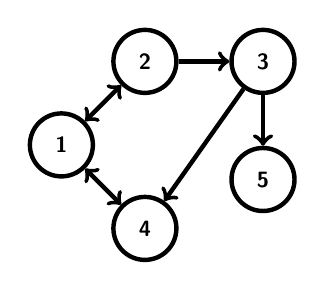
\begin{tikzpicture}[baseline=(current bounding box.center), node distance=15mm, ultra thick, 
        main/.style = {circle, draw, minimum size=8mm, font=\footnotesize\sffamily\bfseries}]
    \node[main] (1) {1};
    \node[main] (2) [above right of=1] {2};
    \node[main] (3) [right of=2] {3};
    \node[main] (4) [below right of=1] {4};
    \node[main] (5) [below of=3] {5};
    \draw[<->] (1) -- (2);
    \draw[<->] (1) -- (4);
    \draw[->] (2) -- (3);
    \draw[->] (3) -- (4);
    \draw[->] (3) -- (5);
\end{tikzpicture}

\begin{myproof} La matriz de adyacencia es \(
A = \begin{pmatrix}
0 & 1 & 0 & 1 & 0 \\
1 & 0 & 1 & 0 & 0 \\
0 & 0 & 0 & 1 & 1 \\
1 & 0 & 0 & 0 & 0 \\
0 & 0 & 0 & 0 & 0 \\
\end{pmatrix}
\), calculando $A^{3}$ se tiene que \(
A^3 = \begin{pmatrix}
0 & 2 & 0 & 2 & 1 \\
2 & 0 & 1 & 0 & 0 \\
0 & 1 & 0 & 1 & 0 \\
1 & 0 & 1 & 0 & 1 \\
0 & 0 & 0 & 0 & 0 \\
\end{pmatrix}
\). El elemento (3,2) de $A^3 = 1,$ por lo cual existe 1 camino de longitud 3 de 3 a 2: $3 \to 4 \to 1 \to 2$.
\end{myproof}

\item 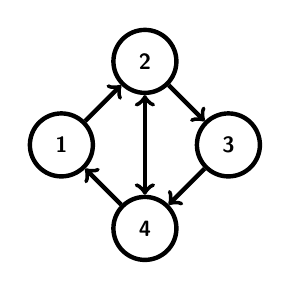
\begin{tikzpicture}[baseline=(current bounding box.center), auto, node distance=1.5cm, ultra thick, 
        main node/.style={circle, draw, minimum size=8mm, font=\footnotesize\sffamily\bfseries}]
    \node[main node] (1) {1};
    \node[main node] (2) [above right of=1] {2};
    \node[main node] (3) [below right of=2] {3};
    \node[main node] (4) [below right of=1] {4};
    \draw[->] (1) -- (2);
    \draw[<-] (1) -- (4);
    \draw[->] (2) -- (3);
    \draw[<->] (2) -- (4);
    \draw[->] (3) -- (4);
\end{tikzpicture}

\begin{myproof} La matriz de adyacencia es \(
B = \begin{pmatrix}
0 & 1 & 0 & 0 \\
0 & 0 & 1 & 1 \\
0 & 0 & 0 & 1 \\
1 & 1 & 0 & 0 \\
\end{pmatrix}
\), donde \(B^3 = \begin{pmatrix}
1 & 1 & 0 & 1 \\
1 & 2 & 1 & 1 \\
0 & 1 & 1 & 1 \\
1 & 1 & 1 & 2 \\
\end{pmatrix}\). Así la posición $(3,2)$ de $B^3$ es $1$ y el camino de longitud 3 de 3 a 2 es \( 3 \to 4 \to 1 \to 2 .\)
\end{myproof}

\item 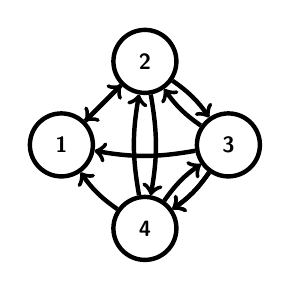
\begin{tikzpicture}[baseline=(current bounding box.center), auto, node distance=1.5cm, ultra thick, 
        main node/.style={circle, draw, minimum size=8mm, font=\footnotesize\sffamily\bfseries}]
    \node[main node] (1) {1};
    \node[main node] (2) [above right of=1] {2};
    \node[main node] (3) [below right of=2] {3};
    \node[main node] (4) [below right of=1] {4};
    \draw[->] (1) -- (2);
    \draw[->] (2) -- (1);
    \draw[->] (2) to [bend left=10] (3);
    \draw[->] (2) to [bend left=10] (4);
    \draw[->] (3) to [bend left=10] (1);
    \draw[->] (3) to [bend left=10] (2);
    \draw[->] (3) to [bend left=10] (4);
    \draw[->] (4) to [bend left=10] (1);
    \draw[->] (4) to [bend left=10] (2);
    \draw[->] (4) to [bend left=10] (3);
    \draw[->] (3) to [bend left=10] (4);  % Corrección: solo una arista 3→4
\end{tikzpicture}

\begin{myproof} La matriz de adyacencia es \(
C = \begin{pmatrix}
0 & 1 & 0 & 0 \\
1 & 0 & 1 & 1 \\
1 & 1 & 0 & 1 \\
1 & 1 & 1 & 0 \\
\end{pmatrix}
,\) donde \(C^3 = \begin{pmatrix}
2 & 2 & 1 & 1 \\
5 & 4 & 4 & 3 \\
5 & 5 & 3 & 4 \\
5 & 5 & 4 & 3 \\
\end{pmatrix}\) por lo cual $C^3_{3,2} = 5.$ Así, existen $5$ caminos de longitud 3 de 3 a 2:
\begin{enumerate}[1.]
\item $3 \to 2 \to 1 \to 2$
\item $3 \to 2 \to 3 \to 2$
\item $3 \to 2 \to 4 \to 2$
\item $3 \to 4 \to 1 \to 2$
\item $3 \to 4 \to 3 \to 2$
\end{enumerate}
\end{myproof}
\end{enumerate}
\end{prob}


\begin{prob} 
Dibuje el grafo para cada matriz de adyacencia:
\begin{enumerate}[a)]
\item $\begin{pmatrix}
2 & 0 & 2 & 4 \\
1 & 4 & 0 & 1 \\
0 & 1 & 3 & 0 \\
2 & 5 & 1 & 3 \\
\end{pmatrix}$

\begin{myproof}
Grafo con 4 vértices $\{1,2,3,4\}$:
\begin{itemize}
\item Bucles: $1\to1$ (2 veces), $2\to2$ (4 veces), $3\to3$ (3 veces), $4\to4$ (3 veces)
\item Aristas múltiples: 
  \begin{itemize}
  \item $1\to3$ (2 aristas)
  \item $1\to4$ (4 aristas)
  \item $2\to1$ (1 arista)
  \item $2\to4$ (1 arista)
  \item $3\to2$ (1 arista)
  \item $4\to1$ (2 aristas)
  \item $4\to2$ (5 aristas)
  \item $4\to3$ (1 arista)
  \end{itemize}
\end{itemize}

\begin{figure}[H]
\centering
\begin{tikzpicture}[->, >=Stealth, shorten >=1pt, node distance=3cm, 
   main/.style = {draw, circle, minimum size=8mm, thick}]
   
\node[main] (1) at (0,0) {1};
\node[main] (2) at (4,0) {2};
\node[main] (3) at (0,-3) {3};
\node[main] (4) at (4,-3) {4};

% Bucles
\foreach \i in {1,2} {
  \draw[->] (1) to [loop above, min distance=8mm, out=70, in=110, looseness=6] (1);
}
\foreach \i in {1,...,4} {
  \draw[->] (2) to [loop above, min distance=8mm, out=70, in=110, looseness=6] (2);
}
\foreach \i in {1,2,3} {
  \draw[->] (3) to [loop left, min distance=8mm, out=160, in=200, looseness=6] (3);
}
\foreach \i in {1,2,3} {
  \draw[->] (4) to [loop right, min distance=8mm, out=-20, in=20, looseness=6] (4);
}

% Aristas 1→3 (2)
\draw[->] (1) to [bend right=10] (3);
\draw[->] (1) to [bend left=10] (3);

% Aristas 1→4 (4)
\foreach \i in {1,...,4} {
  \draw[->] (1) to [bend right=\i*5+10] (4);
}

% Aristas 2→1 (1)
\draw[->] (2) to [bend left=20] (1);

% Aristas 2→4 (1)
\draw[->] (2) to [bend right=20] (4);

% Aristas 3→2 (1)
\draw[->] (3) to [bend left=20] (2);

% Aristas 4→1 (2)
\draw[->] (4) to [bend right=20] (1);
\draw[->] (4) to [bend left=20] (1);

% Aristas 4→2 (5)
\foreach \i in {1,...,5} {
  \draw[->] (4) to [bend left=\i*5] (2);
}

% Aristas 4→3 (1)
\draw[->] (4) to [bend right=20] (3);
\end{tikzpicture}
\caption{Grafo del problema (a)}
\end{figure}
\end{myproof}

\item $\begin{pmatrix}
0 & 0 & 2 & 0 \\
1 & 0 & 0 & 1 \\
0 & 1 & 3 & 0 \\
2 & 5 & 1 & 3 \\
\end{pmatrix}$

\begin{myproof}
Grafo con 4 vértices $\{1,2,3,4\}$:
\begin{itemize}
\item Bucles: $3\to3$ (3 veces), $4\to4$ (3 veces)
\item Aristas múltiples: 
  \begin{itemize}
  \item $1\to3$ (2 aristas)
  \item $2\to1$ (1 arista)
  \item $2\to4$ (1 arista)
  \item $3\to2$ (1 arista)
  \item $4\to1$ (2 aristas)
  \item $4\to2$ (5 aristas)
  \item $4\to3$ (1 arista)
  \end{itemize}
\end{itemize}

\begin{figure}[H]
\centering
\begin{tikzpicture}[->, >=Stealth, shorten >=1pt, node distance=3cm, 
   main/.style = {draw, circle, minimum size=8mm, thick}]
   
\node[main] (1) at (0,0) {1};
\node[main] (2) at (4,0) {2};
\node[main] (3) at (0,-3) {3};
\node[main] (4) at (4,-3) {4};

% Bucles
\foreach \i in {1,2,3} {
  \draw[->] (3) to [loop left, min distance=8mm, out=160, in=200, looseness=6] (3);
}
\foreach \i in {1,2,3} {
  \draw[->] (4) to [loop right, min distance=8mm, out=-20, in=20, looseness=6] (4);
}

% Aristas 1→3 (2)
\draw[->] (1) to [bend right=10] (3);
\draw[->] (1) to [bend left=10] (3);

% Aristas 2→1 (1)
\draw[->] (2) to [bend left=20] (1);

% Aristas 2→4 (1)
\draw[->] (2) to [bend right=20] (4);

% Aristas 3→2 (1)
\draw[->] (3) to [bend left=20] (2);

% Aristas 4→1 (2)
\draw[->] (4) to [bend right=20] (1);
\draw[->] (4) to [bend left=20] (1);

% Aristas 4→2 (5)
\foreach \i in {1,...,5} {
  \draw[->] (4) to [bend left=\i*5] (2);
}

% Aristas 4→3 (1)
\draw[->] (4) to [bend right=20] (3);
\end{tikzpicture}
\caption{Grafo del problema (b)}
\end{figure}
\end{myproof}

\item $\begin{pmatrix}
1 & 0 & 2 & 0 \\
1 & 0 & 2 & 1 \\
0 & 1 & 3 & 0 \\
2 & 5 & 1 & 2 \\
\end{pmatrix}$

\begin{myproof}
Grafo con 4 vértices $\{1,2,3,4\}$:
\begin{itemize}
\item Bucles: $1\to1$ (1 vez), $3\to3$ (3 veces), $4\to4$ (2 veces)
\item Aristas múltiples: 
  \begin{itemize}
  \item $1\to3$ (2 aristas)
  \item $2\to1$ (1 arista)
  \item $2\to3$ (2 aristas)
  \item $2\to4$ (1 arista)
  \item $3\to2$ (1 arista)
  \item $4\to1$ (2 aristas)
  \item $4\to2$ (5 aristas)
  \item $4\to3$ (1 arista)
  \end{itemize}
\end{itemize}

\begin{figure}[H]
\centering
\begin{tikzpicture}[->, >=Stealth, shorten >=1pt, node distance=3cm, 
   main/.style = {draw, circle, minimum size=8mm, thick}]
   
\node[main] (1) at (0,0) {1};
\node[main] (2) at (4,0) {2};
\node[main] (3) at (0,-3) {3};
\node[main] (4) at (4,-3) {4};

% Bucles
\draw[->] (1) to [loop above, min distance=8mm, out=70, in=110, looseness=6] (1);
\foreach \i in {1,2,3} {
  \draw[->] (3) to [loop left, min distance=8mm, out=160, in=200, looseness=6] (3);
}
\foreach \i in {1,2} {
  \draw[->] (4) to [loop right, min distance=8mm, out=-20, in=20, looseness=6] (4);
}

% Aristas 1→3 (2)
\draw[->] (1) to [bend right=10] (3);
\draw[->] (1) to [bend left=10] (3);

% Aristas 2→1 (1)
\draw[->] (2) to [bend left=20] (1);

% Aristas 2→3 (2)
\draw[->] (2) to [bend right=10] (3);
\draw[->] (2) to [bend left=10] (3);

% Aristas 2→4 (1)
\draw[->] (2) to [bend right=20] (4);

% Aristas 3→2 (1)
\draw[->] (3) to [bend left=20] (2);

% Aristas 4→1 (2)
\draw[->] (4) to [bend right=20] (1);
\draw[->] (4) to [bend left=20] (1);

% Aristas 4→2 (5)
\foreach \i in {1,...,5} {
  \draw[->] (4) to [bend left=\i*5] (2);
}

% Aristas 4→3 (1)
\draw[->] (4) to [bend right=20] (3);
\end{tikzpicture}
\caption{Grafo del problema (c)}
\end{figure}
\end{myproof}
\end{enumerate}
\end{prob}



\begin{prob} 
Una aerolínea ofrece vuelos directos entre múltiples ciudades de América Latina. Las ciudades son: Buenos Aires (BA), Sao Paulo (SP), Lima, Bogotá (Bog), Santiago (Stgo), Caracas (Carc) y Ciudad de México (CDMX). Las rutas bidireccionales son:
\begin{itemize}
\item Buenos Aires - Sao Paulo
\item Buenos Aires - Santiago
\item Sao Paulo - Lima
\item Lima - Bogotá
\item Santiago - Lima
\item Bogotá - Caracas
\item Caracas - Ciudad de México
\end{itemize}

Si se representa cada ciudad como un nodo en un grafo y cada vuelo directo como una arista entre dos nodos:
\begin{enumerate}[i.]
\item ¿Cuál es el número mínimo de conexiones necesarias para viajar de una ciudad a otra?
\item ¿Cuál es el número mínimo de conexiones necesarias para viajar desde Buenos Aires a Ciudad de México?
\item ¿Cuál es el número mínimo de conexiones necesarias para viajar desde Bogotá a Sao Paulo?
\end{enumerate}

\begin{myproof}
Grafo no dirigido (todas las rutas son bidireccionales):

\begin{figure}[H]
\centering
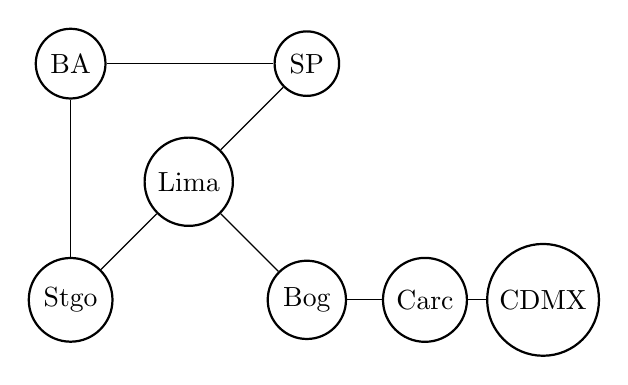
\begin{tikzpicture}[node distance=2.5cm, main/.style={circle, draw, thick, minimum size=8mm}]
\node[main] (BA) at (0,0) {BA};
\node[main] (SP) at (3,0) {SP};
\node[main] (Lima) at (1.5,-1.5) {Lima};
\node[main] (Bog) at (3,-3) {Bog};
\node[main] (Stgo) at (0,-3) {Stgo};
\node[main] (Carc) at (4.5,-3) {Carc};
\node[main] (CDMX) at (6,-3) {CDMX};

\draw (BA) -- (SP);
\draw (BA) -- (Stgo);
\draw (SP) -- (Lima);
\draw (Lima) -- (Bog);
\draw (Stgo) -- (Lima);
\draw (Bog) -- (Carc);
\draw (Carc) -- (CDMX);
\end{tikzpicture}
\caption{Red de vuelos de la aerolínea}
\end{figure}

\begin{enumerate}[i.]
\item \textbf{Distancia máxima (diámetro):} 
La ruta más larga es BA $\to$ Stgo $\to$ Lima $\to$ Bog $\to$ Carc $\to$ CDMX (4 conexiones). 
El diámetro del grafo es 4.

\item \textbf{BA a CDMX:} 
Camino mínimo: BA $\to$ SP $\to$ Lima $\to$ Bog $\to$ Carc $\to$ CDMX (4 conexiones) \\
Otra ruta: BA $\to$ Stgo $\to$ Lima $\to$ Bog $\to$ Carc $\to$ CDMX (4 conexiones) \\
Mínimo: 4 conexiones

\item \textbf{Bogotá a Sao Paulo:} 
Camino mínimo: Bog $\to$ Lima $\to$ SP (2 conexiones)
\end{enumerate}

\begin{itemize}
\item \textbf{Distancia máxima (diámetro):} 5 conexiones (ej: Stgo a CDMX)
\item \textbf{BA a CDMX:} Mínimo \fbox{5} conexiones: BA $\to$ SP $\to$ Lima $\to$ Bog $\to$ Carc $\to$ CDMX
\item \textbf{Bogotá a SP:} Mínimo \fbox{2} conexiones: Bog $\to$ Lima $\to$ SP
\end{itemize}

\begin{table}[H]
\centering
\begin{tabular}{c|c|c}
\textbf{Ruta} & \textbf{Conexiones} & \textbf{Ciudades intermedias} \\
\hline
BA $\to$ CDMX & 5 & BA-SP-Lima-Bog-Carc-CDMX \\
Stgo $\to$ CDMX & 4 & Stgo-Lima-Bog-Carc-CDMX \\
Bog $\to$ SP & 2 & Bog-Lima-SP \\
BA $\to$ Carc & 4 & BA-SP-Lima-Bog-Carc \\
\end{tabular}
\caption{Rutas mínimas entre ciudades}
\end{table}
\end{myproof}
\end{prob}

\begin{prob} 
Una tienda de computadores vende tres tipos de productos: procesadores (\$750.000), tarjetas gráficas (\$950.000) y gabinetes (\$200.000). La tabla muestra las ventas de los primeros cuatro meses:

\begin{table}[H]\centering
\begin{tabular}{|c||c|c|c|}\hline
& Procesadores & Tarjetas gráficas & Gabinetes\\\hline
Enero & 3 & 4 & 3\\
Febrero & 5 & 6 & 0\\
Marzo & 2 & 9 & 4\\
Abril & 1 & 1 & 7\\\hline
\end{tabular}
\end{table}

Escriba una matriz que represente la cantidad total de dinero obtenido cada mes.
\end{prob}

\begin{myproof}
Sea $P = \begin{pmatrix} 750000 \\ 950000 \\ 200000 \end{pmatrix}$ el vector de precios unitarios. La matriz de ventas $V = \begin{pmatrix}
3 & 4 & 3 \\
5 & 6 & 0 \\
2 & 9 & 4 \\
1 & 1 & 7 
\end{pmatrix}$ representa las unidades vendidas por mes (filas = meses, columnas = productos). De esta manera la matriz de ingresos totales por mes se obtiene multiplicando $V$ por $P$. Calculando detalladamente:
\[
\begin{pmatrix}
3 & 4 & 3 \\
5 & 6 & 0 \\
2 & 9 & 4 \\
1 & 1 & 7 
\end{pmatrix}
\begin{pmatrix}
750000 \\ 950000 \\ 200000
\end{pmatrix}
= \begin{pmatrix}
3\cdot750000 + 4\cdot950000 + 3\cdot200000 \\
5\cdot750000 + 6\cdot950000 + 0\cdot200000 \\
2\cdot750000 + 9\cdot950000 + 4\cdot200000 \\
1\cdot750000 + 1\cdot950000 + 7\cdot200000
\end{pmatrix}
\]
\begin{align*}
\text{Enero:}  & \quad 3(750000) + 4(950000) + 3(200000) = 2\,250\,000 + 3\,800\,000 + 600\,000 = 6\,650\,000 \\
\text{Febrero:} & \quad 5(750000) + 6(950000) + 0(200000) = 3\,750\,000 + 5\,700\,000 = 9\,450\,000 \\
\text{Marzo:}  & \quad 2(750000) + 9(950000) + 4(200000) = 1\,500\,000 + 8\,550\,000 + 800\,000 = 10\,850\,000 \\
\text{Abril:}  & \quad 1(750000) + 1(950000) + 7(200000) = 750\,000 + 950\,000 + 1\,400\,000 = 3\,100\,000
\end{align*}

La matriz de ingresos totales por mes es \(
\boxed{\begin{pmatrix}
6\,650\,000 \\
9\,450\,000 \\
10\,850\,000 \\
3\,100\,000
\end{pmatrix}}
\)
\end{myproof}

\begin{prob} 
Un restaurante ofrece tres tipos de platos: vegetarianos (\$5000), carne (\$13000) y mariscos (\$20000). La tabla muestra las ventas mensuales:

\begin{table}[H]\centering
\begin{tabular}{|c||c|}\hline
Tipo de plato & Cant. vendida \\\hline
Vegetariano & 200 \\
Carne & 150 \\
Mariscos & 100 \\\hline
\end{tabular}
\end{table}

Si los costos de producción por plato son: Vegetariano \$3000, Carne \$9000 y Mariscos \$15000, calcule:
\begin{enumerate}[$(a)$]
\item Matriz de costo de producción unitario
\item Matriz de ingresos por tipo de plato
\item Costo total de producción mensual
\item Ingreso total mensual
\item Ganancias mensuales
\end{enumerate}
\end{prob}

\begin{myproof}
\begin{enumerate}[$(a)$]
\item Matriz de costo unitario (vector columna):
\[
C_{\text{unit}} = \begin{pmatrix}
3000 \\
9000 \\
15000
\end{pmatrix}
\]

\item Matriz de ingresos por tipo (precio unitario $\times$ cantidad):
\[
I_{\text{tipo}} = \begin{pmatrix}
5000 \times 200 \\
13000 \times 150 \\
20000 \times 100
\end{pmatrix} = \begin{pmatrix}
1\,000\,000 \\
1\,950\,000 \\
2\,000\,000
\end{pmatrix}
\]

\item Costo total de producción (suma de costos unitarios $\times$ cantidad):
\begin{align*}
&(3000 \times 200) + (9000 \times 150) + (15000 \times 100) \\
&= 600\,000 + 1\,350\,000 + 1\,500\,000 = \boxed{3\,450\,000}
\end{align*}

\item Ingreso total (suma de ingresos por tipo):
\[
1\,000\,000 + 1\,950\,000 + 2\,000\,000 = \boxed{4\,950\,000}
\]

\item Ganancias (ingreso total - costo total):
\[
4\,950\,000 - 3\,450\,000 = \boxed{1\,500\,000}
\]
\end{enumerate}
\end{myproof}

\begin{prob} 
Un vendedor de frutas tiene tres puestos: Plaza Satélite, Plaza Central y San Francisco. Se registraron las ventas de manzanas, naranjas y plátanos en dos períodos de la misma semana:

\begin{table}[H]\centering
\begin{tabular}{|c||c|c|c|} \hline
& Manzanas & Naranjas & Plátanos \\ \hline
Plaza Satélite & 40 & 25 & 30 \\ 
Plaza Central & 15 & 50 & 20 \\ 
San Francisco & 20 & 30 & 25 \\ \hline
\end{tabular}
\caption{Ventas de fruta en los primeros 3 días}
\end{table}

\begin{table}[H]\centering
\begin{tabular}{|c||c|c|c|} \hline
& Manzanas & Naranjas & Plátanos \\ \hline
Plaza Satélite & 25 & 30 & 20 \\ 
Plaza Central & 35 & 15 & 30 \\ 
San Francisco & 45 & 20 & 25 \\ \hline
\end{tabular}
\caption{Ventas de fruta en los últimos 4 días}
\end{table}
Calcule:
\begin{enumerate}[$(a)$]
\item El número de manzanas, naranjas y plátanos vendidos en Plaza Central durante la semana.
\item Puesto donde se vendieron más más plátanos durante cada periodo de la semana.
\item Puesto donde se vendió más fruta en toda la semana.
\item La matriz que representa la venta total de frutas durante toda la semana.
\item Suponga que el vendedor cobra $\$2000$ por cada manzana, $\$300$ por cada naranja y $\$400$ por cada plátano. Encuentre la matriz que representa el ingreso semanal por puesto de venta.
\item ¿Cuál fue el ingreso total por la venta de frutas en toda la semana?
\end{enumerate}
\end{prob}

\begin{myproof}
Defina las matrices de ventas \(
V_1 = \begin{pmatrix}
40 & 25 & 30 \\
15 & 50 & 20 \\
20 & 30 & 25
\end{pmatrix}, \quad 
V_2 = \begin{pmatrix}
25 & 30 & 20 \\
35 & 15 & 30 \\
45 & 20 & 25
\end{pmatrix}
,\) donde las filas representan los puestos (Satélite, Central, San Francisco) y las columnas la cantidad de frutas (manzanas, naranjas, plátanos). Haciendo los cálculos:

\begin{enumerate}[$(a)$]
\item Las ventas en la Plaza Central están en la fila 2
\[
\text{Total} = \begin{pmatrix} 15 \\ 50 \\ 20 \end{pmatrix} + \begin{pmatrix} 35 \\ 15 \\ 30 \end{pmatrix} = \begin{pmatrix} 50 \\ 65 \\ 50 \end{pmatrix}
\]
Se vendieron 50 manzanas, 65 naranjas, 50 plátanos.

\item Los plátanos están en la columna 3, así en el primer período: $\begin{pmatrix} 30 \\ 20 \\ 25 \end{pmatrix}$ se tiene un máximo en Plaza Satélite, mientras que en el segundo período: $\begin{pmatrix} 20 \\ 30 \\ 25 \end{pmatrix}$ se tiene un máximo en Plaza Central (30).

\item La matriz de venta de fruta en total es 
\(
\text{Total por puesto} = \left(V_1 + V_2\right) \begin{pmatrix} 1 \\ 1 \\ 1 \end{pmatrix} = \begin{pmatrix}
65 & 55 & 50 \\
50 & 65 & 50 \\
65 & 50 & 50
\end{pmatrix} \begin{pmatrix} 1 \\ 1 \\ 1 \end{pmatrix} = \begin{pmatrix} 170 \\ 165 \\ 165 \end{pmatrix}
\) por lo que se vendió más fruta en la Plaza Satélite (170 frutas).

\item La matriz de venta total es:
\[
V_{\text{total}} = V_1 + V_2 = \begin{pmatrix}
65 & 55 & 50 \\
50 & 65 & 50 \\
65 & 50 & 50
\end{pmatrix}
\]

\item La matriz de ingresos por puesto se calcula según el vector de precios: $P = \begin{pmatrix} 2000 \\ 300 \\ 400 \end{pmatrix}$
\[
\text{Ingresos} = V_{\text{total}} \cdot P = \begin{pmatrix}
65 & 55 & 50 \\
50 & 65 & 50 \\
65 & 50 & 50
\end{pmatrix} \begin{pmatrix} 2000 \\ 300 \\ 400 \end{pmatrix} = \begin{pmatrix}
65\cdot2000 + 55\cdot300 + 50\cdot400 \\
50\cdot2000 + 65\cdot300 + 50\cdot400 \\
65\cdot2000 + 50\cdot300 + 50\cdot400
\end{pmatrix} = \begin{pmatrix}
166\,500 \\
139\,500 \\
165\,000
\end{pmatrix}
\]

\item \textbf{Ingreso total semanal:}
\[
166\,500 + 139\,500 + 165\,000 = \boxed{471\,000}
\]
\end{enumerate}
\end{myproof}
\section{Matrices invertibles}

\begin{definition}[Matriz invertible]
Una matriz cuadrada $A$ de orden $n \times n$ se dice \textbf{invertible} (o \textbf{no singular}) si existe una matriz $B$ de orden $n \times n$ tal que:
$$AB = BA = I_n$$
donde $I_n$ es la matriz identidad de orden $n$. La matriz $B$ se llama la \textbf{inversa} de $A$ y se denota por $A^{-1}$.
\end{definition}

\begin{example}
Considere la matriz $A = \begin{pmatrix} 2 & 1 \\ 3 & 2 \end{pmatrix}$, esta matriz es invertible pues $A^{-1}= \begin{pmatrix} 2 & -1 \\ -3 & 2 \end{pmatrix},$ ya que $AA^{-1} = I_2,$ detalladamente:
$$\begin{pmatrix} 2 & 1 \\ 3 & 2 \end{pmatrix} \begin{pmatrix} 2 & -1 \\ -3 & 2 \end{pmatrix} = \begin{pmatrix} 4-3 & -2+2 \\ 6-6 & -3+4 \end{pmatrix} = \begin{pmatrix} 1 & 0 \\ 0 & 1 \end{pmatrix}.$$
\end{example}

\begin{theorem}
Los dos métodos fundamentales para calcular la matriz inversa son:
\begin{enumerate}
\item \textbf{Eliminación de Gauss-Jordan, Lema \ref{lem:gauss-jordan}:} Mediante operaciones elementales de fila, transforma la matriz aumentada $[A|I]$ en $[I|A^{-1}]$. 
\item \textbf{Matriz adjunta, Teorema \ref{thm:adjunta}:} Emplea la fórmula $A^{-1} = \frac{1}{\det(A)} \cdot \operatorname{adj}(A)$, requiriendo el cálculo de determinantes y cofactores.
\end{enumerate}
Ambos requieren una fundamentación teórica sólida, esencial en álgebra lineal, que desarrollaremos a continuación. Todo se basa en el texto \cite{araujo2014algebra}.
\end{theorem}
\subsection{Matrices invertibles: Método de eliminación gaussiana}

\begin{definition}[Operaciones elementales de fila]
Son transformaciones reversibles sobre las filas definidas así:
\begin{enumerate}
\item \textbf{Combinación lineal:} $k f_i + f_j \to f_j$ \\
  (Multiplicar la fila $i$ por $k$ y sumar a la fila $j$ para cambiar $f_j$)
  
\item \textbf{Escalamiento:} $k \cdot f_i \to f_i$ \quad ($k \neq 0$) \\
  (Multiplicar la fila $i$ por $k$)

\item \textbf{Intercambio:} $f_i \leftrightarrow f_j$ \\
  (Intercambiar filas $i$ y $j$)
\end{enumerate}
\end{definition}

\begin{example}
Sea $A = \begin{pmatrix} 1 & 2 \\ 3 & 4 \\ 5 & 6 \end{pmatrix},$ algunas operaciones elementales de fila son:
\begin{myproof}
\begin{enumerate}
\item Multiplicar por -3 la fila 1 y sumar a la fila 2 para cambiar la fila 2, $(-3)f_1 + f_2 \to f_2$: 
  $\begin{pmatrix} 1 & 2 \\ 0 & -2 \\ 5 & 6 \end{pmatrix}.$
\item Multiplicar la fila 2 por 0.5, $0.5 \cdot f_2 \to f_2$: 
  $\begin{pmatrix} 1 & 2 \\ 0 & -1 \\ 5 & 6 \end{pmatrix}$
\item Intercambiar la fila 1 con la fila 3, $f_1 \leftrightarrow f_3$: 
  $\begin{pmatrix} 5 & 6 \\ 0 & -1 \\ 1 & 2 \end{pmatrix}$
\end{enumerate}
\end{myproof}
\end{example}

\begin{rem}\label{rem:prop-elementales}
Cada operación tiene inversa:
  \begin{itemize}
  \item $k f_i + f_j \to f_j$ $\Rightarrow$ $-k f_i + f_j \to f_j.$
  \item $k \cdot f_i \to f_i$ $\Rightarrow$ $\frac{1}{k} \cdot f_i \to f_i.$
  \item $f_i \leftrightarrow f_j$ $\Rightarrow$ $f_i \leftrightarrow f_j$ (misma operación).
  \end{itemize}
\end{rem}

\begin{definition}[Matriz elemental]
Una matriz elemental $E$ de orden $n \times n$ es la matriz obtenida al aplicar \textbf{una operación elemental de fila} a la matriz identidad $I_n$. Existen tres tipos:

\begin{enumerate}
\item \textbf{Combinación:} Resultado de $k f_i + f_j \to f_j$ en $I_n.$ 
  
\item \textbf{Escalamiento:} Resultado de $k \cdot f_i \to f_i$ en $I_n$ 
  
\item \textbf{Intercambio:} Resultado de $f_i \leftrightarrow f_j$ en $I_n$ 
\end{enumerate}
\end{definition}

\begin{example} Algunas matrices elementales son:
\begin{enumerate}
\item $k f_1 + f_2 \to f_2$ en $I_2$: $E = \begin{pmatrix} 1 & 0 \\ k & 1 \end{pmatrix}$
\item $k \cdot f_2 \to f_2$ en $I_3$: $E = \begin{pmatrix} 1 & 0 & 0 \\ 0 & k & 0 \\ 0 & 0 & 1 \end{pmatrix}$
\item $f_1 \leftrightarrow f_2$ en $I_3:$ $E = \begin{pmatrix} 0 & 1 & 0 \\ 1 & 0 & 0 \\ 0 & 0 & 1 \end{pmatrix}$
\end{enumerate}
\end{example}

\begin{theorem} Las propiedades fundamentales de las matrices elementales son
\begin{enumerate}

\item Cada operación elemental $k f_i + f_j \to f_j$ aplicada a $A$ equivale a $E \cdot A$
\item La inversa de una matriz elemental corresponde a la operación inversa, es decir:
  \begin{itemize}
  \item $E_{\text{comb}}^{-1}$: $-k f_i + f_j \to f_j$
  \item $E_{\text{esc}}^{-1}$: $\frac{1}{k} \cdot f_i \to f_i$
  \item $E_{\text{int}}^{-1}$: $f_i \leftrightarrow f_j$
  \end{itemize}
\end{enumerate}
\end{theorem}

\begin{definition}[Matrices equivalentes por filas]
Dos matrices $A$ y $B$ son equivalentes por filas $$A \sim_f B$$ si $B$ se obtiene de $A$ mediante una secuencia finita de operaciones elementales de fila:
\(A \xrightarrow{\text{op}_1} A_1 \xrightarrow{\text{op}_2} \cdots \xrightarrow{\text{op}_k} B \)  o equivalentemente \( B = E_k \cdots E_1 A
\)
donde cada  operación $\text{op}_i$ es de la forma $k f_p + f_q \to f_q$, $k \cdot f_r \to f_r$, o $f_s \leftrightarrow f_t$.
\end{definition}

\begin{example}\label{ex:equiv}
Sea $A = \begin{pmatrix} 1 & 3 \\ 2 & 4 \end{pmatrix}$. Verifique que es equivalente a la matriz $B = \begin{pmatrix} 1 & 3 \\ 0 & -2 \end{pmatrix}$.
\begin{myproof}
Aplicando $(-2)f_1 + f_2 \to f_2$ se tiene que $\begin{pmatrix} 1 & 3 \\ 2-2(1) & 4-2(3) \end{pmatrix} = \begin{pmatrix} 1 & 3 \\ 0 & -2 \end{pmatrix} = B,$ por lo cual la matriz elemental correspondiente es $E = \begin{pmatrix} 1 & 0 \\ -2 & 1 \end{pmatrix}.$ Entonces $EA = B$ y $A \sim_f B$.
\end{myproof}
\end{example}

\begin{example}\label{ex:equiv2}
Determine la secuencia de operaciones para que $A = \begin{pmatrix} 0 & 2 \\ 1 & 0 \end{pmatrix}$ sea equivalente a $B = \begin{pmatrix} 1 & 0 \\ 0 & 1 \end{pmatrix}.$
\begin{myproof}
\begin{enumerate}
\item $f_1 \leftrightarrow f_2$: $\begin{pmatrix} 1 & 0 \\ 0 & 2 \end{pmatrix}$
\item $\frac{1}{2} \cdot f_2 \to f_2$: $\begin{pmatrix} 1 & 0 \\ 0 & 1 \end{pmatrix} = B$
\end{enumerate}
Operaciones: $B = E_2 E_1 A$ donde $E_1 = \begin{pmatrix} 0 & 1 \\ 1 & 0 \end{pmatrix}$ (intercambio), $E_2 = \begin{pmatrix} 1 & 0 \\ 0 & 0.5 \end{pmatrix}$ (escalamiento).
\end{myproof}
\end{example}


\begin{definition}[Matriz diagonal]
Una matriz cuadrada $D = (d_{ij})$ es \textbf{diagonal} si $d_{ij} = 0$ para todo $i \neq j$. Es decir, todos los elementos fuera de la diagonal principal son cero.
\end{definition}

\begin{example} Las matrices 
$\begin{pmatrix}
3 & 0 & 0 \\
0 & -5 & 0 \\
0 & 0 & 1 
\end{pmatrix}$ y $\begin{pmatrix}
a & 0 \\
0 & b 
\end{pmatrix}$ son diagonales.
\end{example}

\begin{definition}[Matriz triangular]
Una matriz cuadrada es:
\begin{itemize}
\item \textbf{Triangular superior:} Elementos bajo la diagonal principal son cero ($a_{ij}=0$ si $i>j$)
\item \textbf{Triangular inferior:} Elementos sobre la diagonal principal son cero ($a_{ij}=0$ si $i<j$)
\end{itemize}
\end{definition}

\begin{example} $\begin{pmatrix} 2 & 9 \\ 0 & 4 \end{pmatrix}$ es una matriz triangular superior y una matriz triangular inferior es $\begin{pmatrix} 1 & 0 \\ 3 & 5 \end{pmatrix}.$
\end{example}

\begin{definition}[Matriz simétrica] Una matriz cuadrada $A$ es \textbf{simétrica} si $A^T = A$ ($a_{ij} = a_{ji}$). Los elementos son simétricos respecto a la diagonal principal.
\end{definition}

\begin{example} La matriz
$\begin{pmatrix}
7 & -1 & 3 \\
-1 & 0 & 4 \\
3 & 4 & 2 
\end{pmatrix}$ es simétrica.
\end{example}

\begin{definition}[Matriz antisimétrica] Una matriz cuadrada $A$ es \textbf{antisimétrica} si $A^T = -A$ ($a_{ij} = -a_{ji}$). Los elementos diagonales son cero.
\end{definition}

\begin{example} Las matrices
$\begin{pmatrix}
0 & 2 \\
-2 & 0 
\end{pmatrix}$ y $\begin{pmatrix}
0 & 1 & -3 \\
-1 & 0 & 4 \\
3 & -4 & 0 
\end{pmatrix}$ son antisimétricas.
\end{example}

\begin{definition}[Traza de una matriz] \label{def:traza}
La traza de una matriz cuadrada $A$ es la suma de sus elementos diagonales, es decir, \( \operatorname{tr}(A) = \sum_{i=1}^n a_{ii} .\)
\end{definition}

\begin{example} Para $B = \begin{pmatrix} 2 & 5 \\ -1 & 3 \end{pmatrix}$, su traza es $\operatorname{tr}(B) = 2 + 3 = 5$.
\end{example}

\begin{theorem}[Algunas propiedades de la traza, las matrices simétricas y antisimétricas]\label{thm:proptraza} Dada una matriz cuadrada $A$, su traza tiene las siguientes propiedades:
\begin{enumerate}
\item \textbf{Traza de antisimétrica:} Si $A$ es antisimétrica, entonces $\operatorname{tr}(A) = 0$
  
\item \textbf{Descomposición simétrica-antisimétrica:} Toda matriz cuadrada $A$ puede expresarse como:
\[
A = \frac{A + A^T}{2} + \frac{A - A^T}{2}
\]
donde $\frac{A + A^T}{2}$ es simétrica y $\frac{A - A^T}{2}$ es antisimétrica.

\item \textbf{Linealidad de traza:} Para matrices $n\times n$ y escalares $\alpha,\beta$:
\[
\operatorname{tr}(\alpha A + \beta B) = \alpha \operatorname{tr}(A) + \beta \operatorname{tr}(B)
\]

\item \textbf{Traza de producto:} $\operatorname{tr}(AB) = \operatorname{tr}(BA)$
\end{enumerate}
\end{theorem}

\begin{proof}
Demostración de (1): Si $A$ es antisimétrica, $a_{ii} = -a_{ii}$ implica $2a_{ii}=0$, luego $a_{ii}=0$. Por tanto $\operatorname{tr}(A) = \sum a_{ii} = 0$.

Demostración de (2): Sea $S = \frac{A + A^T}{2}$, entonces $S^T = \frac{A^T + A}{2} = S$ (simétrica). \\
Sea $K = \frac{A - A^T}{2}$, entonces $K^T = \frac{A^T - A}{2} = -K$ (antisimétrica). \\
Además $S + K = \frac{A + A^T + A - A^T}{2} = A$.
\end{proof}

\begin{example} Descompanga la matriz $A = \begin{pmatrix} 1 & 4 \\ 2 & 3 \end{pmatrix}$ de la forma simétrica-antisimétrica.
\begin{myproof}
\[
\text{Simétrica: } \frac{1}{2}\left( \begin{pmatrix} 1 & 4 \\ 2 & 3 \end{pmatrix} + \begin{pmatrix} 1 & 2 \\ 4 & 3 \end{pmatrix} \right) = \begin{pmatrix} 1 & 3 \\ 3 & 3 \end{pmatrix}
\]
\[
\text{Antisimétrica: } \frac{1}{2}\left( \begin{pmatrix} 1 & 4 \\ 2 & 3 \end{pmatrix} - \begin{pmatrix} 1 & 2 \\ 4 & 3 \end{pmatrix} \right) = \begin{pmatrix} 0 & 1 \\ -1 & 0 \end{pmatrix}
\]
Suma: $\begin{pmatrix} 1 & 3 \\ 3 & 3 \end{pmatrix} + \begin{pmatrix} 0 & 1 \\ -1 & 0 \end{pmatrix} = \begin{pmatrix} 1 & 4 \\ 2 & 3 \end{pmatrix}$
\end{myproof}
\end{example}


\begin{definition}[Forma escalonada]\label{def:escalonada}
Una matriz está en \textbf{forma escalonada} si cumple:
\begin{enumerate}
\item Todas las filas nulas están en la parte inferior.
\item Cada fila no nula tiene pivote (primer elemento $\neq 0$).
\item Los pivotes están desplazados a la derecha en filas inferiores.
\item Hay ceros debajo de cada pivote.
\end{enumerate}
\end{definition}

\begin{example} Verifique si la siguiente matriz está en forma escalonada:
\( \begin{pmatrix}
\boxed{3} & 2 & 0 & -1 & 4 \\
0 & \boxed{5} & 1 & 3 & 0 \\
0 & 0 & 0 & \boxed{2} & 1 \\
0 & 0 & 0 & 0 & 0 \\
\end{pmatrix}
\).

\begin{myproof} Note que la fila nula (cuarta fila) está en la parte inferior y los pivotes de las filas no nulas son: 
  \begin{itemize}
  \item Fila 1: pivote $\boxed{3}$ (columna 1)
  \item Fila 2: pivote $\boxed{5}$ (columna 2)
  \item Fila 3: pivote $\boxed{2}$ (columna 4)
  \end{itemize}
  Además, los pivotes están desplazados a la derecha:
  \begin{itemize}
  \item Fila 1: pivote en columna 1
  \item Fila 2: pivote en columna 2 ($>1$)
  \item Fila 3: pivote en columna 4 ($>2$)
  \end{itemize}
  y debajo de cada pivote hay ceros:
  \begin{itemize}
  \item Debajo de $\boxed{3}$: $a_{21}=0$, $a_{31}=0$, $a_{41}=0$
  \item Debajo de $\boxed{5}$: $a_{32}=0$, $a_{42}=0$
  \item Debajo de $\boxed{2}$: $a_{43}=0$ (aunque $a_{44}=0$ es redundante)
  \end{itemize}
por lo cual la matriz está en la forma escalonada. 

Note que la siguiente matriz \textbf{no} está en forma escalonada: \( \begin{pmatrix}
0 & \boxed{4} & 1 \\
\boxed{2} & 0 & 3 \\
0 & 0 & 0 
\end{pmatrix}
\) pues aunque la fila nula está abajo el  pivote $\boxed{2}$ (fila 2, col 1) está a la izquierda de pivote $\boxed{4}$ (fila 1, col 2) y esto implica que debajo de $\boxed{4}$ hay $0$ (correcto) pero debajo de $\boxed{2}$ no aplica por la violación previa.
\end{myproof}



\end{example}

\begin{definition}[Forma escalonada reducida]\label{def:escalonada-reducida}
Una matriz está en \textbf{forma escalonada reducida} si cumple:
\begin{enumerate}
\item Está en forma escalonada (cumple la definición \ref{def:escalonada})
\item \textbf{Pivotes unitarios:} Cada pivote es 1.
\item \textbf{Ceros sobre pivotes:} En cada columna con pivote, todos los elementos sobre él son cero.
\end{enumerate}
\end{definition}

\begin{example} Verifique si las matrices \(
\begin{pmatrix}
\boxed{1} & 0 & 0 & 2 \\
0 & \boxed{1} & 0 & -3 \\
0 & 0 & \boxed{1} & 4 
\end{pmatrix}, \quad
\begin{pmatrix}
\boxed{1} & 4 & 0 \\
0 & 0 & \boxed{1} \\
0 & 0 & 0 
\end{pmatrix}
\) están en la forma escalonada reducida:


\begin{myproof} Note que los pivotes son 1, además que hay ceros encima y debajo de cada pivote. \end{myproof}
\end{example}

\begin{example} Las siguientes matrices \textbf{No} son forma escalonada reducida:
\[
\begin{pmatrix}
\boxed{2} & 1 \\  % Pivote ≠ 1
0 & \boxed{1}
\end{pmatrix}, \quad
\begin{pmatrix}
\boxed{1} & 3 \\
0 & \boxed{1} \\  % Falta cero sobre pivote inferior
\end{pmatrix}\]
\end{example}

\begin{rem}\label{rem:gauss}
La construcción de matrices escalonadas y escalonadas reducidas conduce a dos algoritmos fundamentales del álgebra lineal:
\begin{itemize}
\item El \textbf{algoritmo de eliminación gaussiana} (Lema \ref{lem:gauss}), que transforma cualquier matriz en forma escalonada mediante operaciones elementales de fila.
\item El \textbf{algoritmo de Gauss-Jordan} (Lema \ref{lem:gauss-jordan}), que extiende este proceso para obtener la forma escalonada reducida única.
\end{itemize}
Estos algoritmos, desarrollados por Carl Friedrich Gauss y Wilhelm Jordan, revolucionaron el álgebra lineal por su:
\begin{itemize}
\item \textbf{Eficiencia computacional:} Complejidad $O(n^3)$ para matrices $n\times n$
\item \textbf{Versatilidad:} Resuelven sistemas lineales, calculan rangos, inversas y determinantes
\item \textbf{Estabilidad numérica:} Con pivoteo, minimizan errores de redondeo
\end{itemize}
Su implementación sistemática se muestra en los Lemas \ref{lem:gauss} y \ref{lem:gauss-jordan}.
\end{rem}

\begin{lemma}[Algoritmo de Eliminación Gaussiana]\label{lem:gauss}
Cualquier matriz se puede convertir en forma escalonada usando las tres operaciones elementales de fila. El proceso funciona así:

\begin{enumerate}
    \item \textbf{Empezar:} Comenzar con la primera fila y la primera columna.
    
    \item \textbf{Buscar un número distinto de cero:} En la columna actual, buscar hacia abajo una entrada que no sea cero para usarla como pivote. Si toda la columna tiene ceros, pasar a la siguiente columna.
    
    \item \textbf{Poner el pivote arriba:} Si el número encontrado no está en la fila que toca, intercambiar esas dos filas.
    
    \item \textbf{Hacer ceros abajo:} Para cada fila que está debajo del pivote, sumarle un múltiplo adecuado de la fila del pivote para que quede cero en esa posición.
    
    \item \textbf{Continuar:} Pasar a la siguiente fila y columna, y repetir todo el proceso hasta terminar la matriz.
\end{enumerate}

Matemáticamente, en el paso 4 se calcula $m_{jk} = \frac{a_{jp}}{a_{kp}}$ y se realiza la operación $ - m_{jk} \cdot f_k + f_j \to f_j $ para cada fila $j$ debajo de la fila pivote $k$.
\end{lemma}

\begin{example}
Reducir $A = \begin{pmatrix} 0 & 2 & 1 \\ 3 & 6 & 3 \\ 2 & 4 & 2 \end{pmatrix}$ a forma escalonada:
\begin{myproof}
\begin{enumerate}
\item Intercambiar $f_1 \leftrightarrow f_2$: $\begin{pmatrix} \boxed{3} & 6 & 3 \\ 0 & 2 & 1 \\ 2 & 4 & 2 \end{pmatrix}$
\item Eliminar debajo: $(-\frac{2}{3})f_1 + f_3 \to f_3$: $\begin{pmatrix} 3 & 6 & 3 \\ 0 & \boxed{2} & 1 \\ 0 & 0 & 0 \end{pmatrix}$
\end{enumerate}
Forma escalonada: $\begin{pmatrix} 3 & 6 & 3 \\ 0 & 2 & 1 \\ 0 & 0 & 0 \end{pmatrix}$
\end{myproof}
\end{example}

\begin{lemma}[Algoritmo de Gauss-Jordan]\label{lem:gauss-jordan}
Este método mejora la eliminación gaussiana para obtener una matriz donde cada pivote vale 1 y tiene ceros tanto arriba como abajo de cada pivote:

\begin{enumerate}
    \item \textbf{Hacer la forma escalonada:} Primero aplicar eliminación gaussiana (Lema \ref{lem:gauss}) para obtener la forma escalonada.
    
    \item \textbf{Convertir pivotes en unos:} Para cada pivote $a_{kp}$ que no sea 1, dividir toda su fila entre ese número usando la operación $\frac{1}{a_{kp}}f_k \to f_k$.
    
    \item \textbf{Limpiar hacia arriba:} Para cada pivote que ya vale 1 y está en la posición $(k,p)$, eliminar todos los números que están arriba de él. Para cada fila $i$ que está por encima (desde $i = 1$ hasta $k-1$), realizar:
    \( - a_{ip} \cdot f_k + f_i\to f_i
    \) donde $a_{ip}$ es el número que queremos convertir en cero.
\end{enumerate}

Al final se obtiene la forma escalonada reducida, donde cada columna pivote tiene un 1 en la posición del pivote y ceros en todas las demás posiciones.
\end{lemma}

\begin{example}
Continuando con $A = \begin{pmatrix} 3 & 6 & 3 \\ 0 & 2 & 1 \\ 0 & 0 & 0 \end{pmatrix}$:
\begin{myproof}
\begin{enumerate}
\item $\frac{1}{3}f_1 \to f_1$: $\begin{pmatrix} 1 & 2 & 1 \\ 0 & 2 & 1 \\ 0 & 0 & 0 \end{pmatrix}$
  
 \item $\frac{1}{2}f_2 \to f_2$: $\begin{pmatrix} 1 & 2 & 1 \\ 0 & 1 & 0.5 \\ 0 & 0 & 0 \end{pmatrix}$
  
\item $(-2)f_2 + f_1 \to f_1$: $\begin{pmatrix} \boxed{1} & 0 & 0 \\ 0 & \boxed{1} & 0.5 \\ 0 & 0 & 0 \end{pmatrix}$
\end{enumerate}
Forma escalonada reducida: $\begin{pmatrix} 1 & 0 & 0 \\ 0 & 1 & 0.5 \\ 0 & 0 & 0 \end{pmatrix}$
\end{myproof}
\end{example}

\begin{theorem}[Unicidad de la forma escalonada reducida]
Toda matriz es equivalente por filas a una \textbf{única} matriz en forma escalonada reducida.

\begin{proof}
Se demuestra mediante el algoritmo de Gauss-Jordan, que aplica operaciones elementales de forma sistemática para alcanzar una matriz única.
\end{proof}
\end{theorem}
\begin{definition}[Rango de una matriz]\label{def:rango}
Sea \( A \) una matriz \( m \times n \). El \textbf{rango} de \( A \), denotado \( \operatorname{rango}(A) \) o \( \operatorname{rank}(A) \), es:
\begin{itemize}
\item El número de filas no nulas en su \textbf{forma escalonada} (Definición \ref{def:escalonada})
\item El número de pivotes en su \textbf{forma escalonada reducida} (Definición \ref{def:escalonada-reducida})
\end{itemize}
\end{definition}

\begin{theorem}[Propiedades fundamentales del rango]\label{thm:rango-prop}
Para cualquier matriz \( A \):
\begin{enumerate}
\item \( 0 \leq \operatorname{rango}(A) \leq \min\{m, n\} \)
\item \( \operatorname{rango}(A) = \operatorname{rango}(A^T) \)
\item \( \operatorname{rango}(AB) \leq \min\{\operatorname{rango}(A), \operatorname{rango}(B)\} \)
\item Si \( P \) y \( Q \) invertibles: \( \operatorname{rango}(PAQ) = \operatorname{rango}(A) \)
\end{enumerate}
\end{theorem}

\begin{example}[Cálculo por eliminación gaussiana]
Sean \( A = \begin{pmatrix}
1 & 2 & 3 \\
2 & 4 & 6 \\
3 & 6 & 9 
\end{pmatrix} \), y \( B = \begin{pmatrix}
1 & 0 & 2 \\
0 & 3 & -1 \\
4 & 0 & 5 
\end{pmatrix} \) calcule su rango.
\begin{myproof}
\begin{enumerate}
\item Para $A:$
\begin{enumerate}
\item \( (-2)f_1 + f_2 \to f_2 \): \(\begin{pmatrix} 1 & 2 & 3 \\ 0 & 0 & 0 \\ 3 & 6 & 9 \end{pmatrix}\)
\item \( (-3)f_1 + f_3 \to f_3 \): \(\begin{pmatrix} \boxed{1} & 2 & 3 \\ 0 & 0 & 0 \\ 0 & 0 & 0 \end{pmatrix}\)
\end{enumerate}
Forma escalonada tiene 1 fila no nula \(\Rightarrow \operatorname{rango}(A) = 1\).

\item Para $B:$
\begin{enumerate}
\item \( (-4)f_1 + f_3 \to f_3 \): \(\begin{pmatrix} 1 & 0 & 2 \\ 0 & \boxed{3} & -1 \\ 0 & 0 & -3 \end{pmatrix}\)
\item Escalonada: \(\begin{pmatrix} \boxed{1} & 0 & 2 \\ 0 & \boxed{3} & -1 \\ 0 & 0 & \boxed{-3} \end{pmatrix}\)
\end{enumerate}
Tres pivotes \(\Rightarrow \operatorname{rango}(B) = 3 = \min\{3,3\}\).
\end{enumerate}
\end{myproof}
\end{example}

\begin{theorem}[Caracterización de matrices invertibles, version 1]\label{thm:invertible-equiv}
Sea $A$ una matriz cuadrada de orden $n \times n$. Las siguientes afirmaciones son equivalentes:
\begin{enumerate}
    \item $A$ es invertible.
    \item La forma escalonada reducida de $A$ es la matriz identidad $I_n$.
    \item $A$ se puede escribir como producto de matrices elementales.
    \item $A$ tiene rango máximo ($\text{rango}(A) = n$).
\end{enumerate}
\end{theorem}

\begin{proof}
Demostraremos las equivalencias siguiendo el ciclo (1) $\Rightarrow$ (2) $\Rightarrow$ (3) $\Rightarrow$ (4) $\Rightarrow$ (5).

\textbf{(1) $\Rightarrow$ (2):} Supongamos que $A$ es invertible. 

Sea $R$ la forma escalonada reducida de $A$. Por definición del algoritmo de Gauss-Jordan, existen matrices elementales $E_1, E_2, \ldots, E_k$ tales que:
\[E_k E_{k-1} \cdots E_1 A = R\]

Como cada matriz elemental es invertible y el producto de matrices invertibles es invertible, la matriz $P = E_k E_{k-1} \cdots E_1$ es invertible. Por tanto, $R = PA$ donde $P$ es invertible.

Dado que $A$ es invertible por hipótesis, el producto $R = PA$ también es invertible (producto de matrices invertibles).

Ahora, $R$ es una matriz en forma escalonada reducida e invertible. Veamos que esto implica $R = I_n$:
\begin{itemize}
    \item Si $R$ tuviera una fila de ceros, entonces $\det(R) = 0$, lo que contradice que $R$ sea invertible.
    \item Como $R$ está en forma escalonada reducida, tiene exactamente $n$ pivotes (uno por fila).
    \item Cada pivote vale 1 y está en una columna diferente.
    \item Como no hay filas nulas, los pivotes deben estar en las posiciones $(1,1), (2,2), \ldots, (n,n)$.
    \item Por la estructura de la forma escalonada reducida, esto significa $R = I_n$.
\end{itemize}

\textbf{(2) $\Rightarrow$ (3):} Si la forma escalonada reducida de $A$ es $I_n$, entonces:
\[E_k E_{k-1} \cdots E_1 A = I_n\]

Multiplicando ambos lados por la izquierda por $(E_k E_{k-1} \cdots E_1)^{-1}$:
\[A = (E_k E_{k-1} \cdots E_1)^{-1} = E_1^{-1} E_2^{-1} \cdots E_k^{-1}\]

Como la inversa de una matriz elemental es también una matriz elemental, $A$ es producto de matrices elementales.

\textbf{(3) $\Rightarrow$ (4):} Si $A$ es producto de matrices elementales, digamos $A = F_1 F_2 \cdots F_m$, entonces:

Las operaciones elementales de fila no cambian el rango de una matriz. Como cada $F_i$ corresponde a una operación elemental, tenemos:
\[\text{rango}(A) = \text{rango}(F_1 F_2 \cdots F_m I_n) = \text{rango}(I_n) = n\]

\textbf{(4) $\Rightarrow$ (1):} Si $\text{rango}(A) = n$, entonces la forma escalonada reducida de $A$ tiene $n$ pivotes, uno en cada fila. Como la matriz es $n \times n$, debe tener la forma $I_n$.

Por el argumento de (2) $\Rightarrow$ (3) $\Rightarrow$ (1), si la forma escalonada reducida es $I_n$, entonces $A$ es producto de matrices elementales, y por tanto invertible.
\end{proof}

\begin{example}
Verificar que $A = \begin{pmatrix} 1 & 2 \\ 3 & 4 \end{pmatrix}$ es invertible mediante su forma escalonada reducida.
\begin{myproof}
\textbf{Paso 1:} Eliminación gaussiana  
Operación: $(-3)f_1 + f_2 \to f_2$  
$A \to \begin{pmatrix} \boxed{1} & 2 \\ 0 & -2 \end{pmatrix}$

\textbf{Paso 2:} Escalonamiento reducido  
a) $\left(-\frac{1}{2}\right) \cdot f_2 \to f_2$: $\begin{pmatrix} 1 & 2 \\ 0 & 1 \end{pmatrix}$  
b) $(-2)f_2 + f_1 \to f_1$: $\begin{pmatrix} \boxed{1} & 0 \\ 0 & \boxed{1} \end{pmatrix} = I_2$

Como se obtuvo $I_2$, $A$ es invertible. Además:  
\[
A = \underbrace{\begin{pmatrix} 1 & 0 \\ 3 & 1 \end{pmatrix}}_{E_1^{-1}} \underbrace{\begin{pmatrix} 1 & 0 \\ 0 & -2 \end{pmatrix}}_{E_2^{-1}} \underbrace{\begin{pmatrix} 1 & -2 \\ 0 & 1 \end{pmatrix}}_{E_3^{-1}}
\]
donde $E_1, E_2, E_3$ corresponden a las operaciones aplicadas.
\end{myproof}
\end{example}

\begin{example}
Matriz no invertible: $B = \begin{pmatrix} 1 & 2 \\ 2 & 4 \end{pmatrix}$  
Operaciones:  
$(-2)f_1 + f_2 \to f_2$: $\begin{pmatrix} \boxed{1} & 2 \\ 0 & 0 \end{pmatrix}$  
Forma escalonada reducida: $\begin{pmatrix} 1 & 2 \\ 0 & 0 \end{pmatrix} \neq I_2$  
Luego $B$ no es invertible.
\end{example}
\begin{prob}\label{ej.inversa} Use el Algoritmo de eliminación gaussiana (Lema \ref{lem:gauss-jordan}) para calcular la inversa de $A=\begin{pmatrix}1&2&3\\2&5&3\\1&0&8 \end{pmatrix}.$

\end{prob}
\begin{myproof}
\textbf{Paso 1:} Formar matriz aumentada \([A|I_3]\):
\[
\left(\begin{array}{ccc|ccc}
1 & 2 & 3 & 1 & 0 & 0 \\
2 & 5 & 3 & 0 & 1 & 0 \\
1 & 0 & 8 & 0 & 0 & 1 \\
\end{array}\right)
\]

\textbf{Paso 2:} Hacer ceros debajo de \(a_{11}\) (pivote=1):
\begin{align*}
& \text{Operación: } (-2)f_1 + f_2 \to f_2 \\
& \text{Operación: } (-1)f_1 + f_3 \to f_3 \\
& \rightarrow \left(\begin{array}{ccc|ccc}
\boxed{1} & 2 & 3 & 1 & 0 & 0 \\
0 & 1 & -3 & -2 & 1 & 0 \\
0 & -2 & 5 & -1 & 0 & 1 \\
\end{array}\right)
\end{align*}

\textbf{Paso 3:} Hacer ceros debajo/encima de \(a_{22}\) (pivote=1):
\begin{align*}
& \text{Operación: } (2)f_2 + f_3 \to f_3 \\
& \rightarrow \left(\begin{array}{ccc|ccc}
1 & 2 & 3 & 1 & 0 & 0 \\
0 & \boxed{1} & -3 & -2 & 1 & 0 \\
0 & 0 & -1 & -5 & 2 & 1 \\
\end{array}\right)
\end{align*}

\textbf{Paso 4:} Normalizar fila 3 (pivote= -1):
\begin{align*}
& \text{Operación: } (-1) \cdot f_3 \to f_3 \\
& \rightarrow \left(\begin{array}{ccc|ccc}
1 & 2 & 3 & 1 & 0 & 0 \\
0 & 1 & -3 & -2 & 1 & 0 \\
0 & 0 & \boxed{1} & 5 & -2 & -1 \\
\end{array}\right)
\end{align*}

\textbf{Paso 5:} Hacer ceros encima de \(a_{33}\):
\begin{align*}
& \text{Operación: } (3)f_3 + f_2 \to f_2 \\
& \text{Operación: } (-3)f_3 + f_1 \to f_1 \\
& \rightarrow \left(\begin{array}{ccc|ccc}
1 & 2 & 0 & -14 & 6 & 3 \\
0 & 1 & 0 & 13 & -5 & -3 \\
0 & 0 & 1 & 5 & -2 & -1 \\
\end{array}\right)
\end{align*}

\textbf{Paso 6:} Hacer ceros encima de \(a_{22}\):
\begin{align*}
& \text{Operación: } (-2)f_2 + f_1 \to f_1 \\
& \rightarrow \left(\begin{array}{ccc|ccc}
\boxed{1} & 0 & 0 & -40 & 16 & 9 \\
0 & \boxed{1} & 0 & 13 & -5 & -3 \\
0 & 0 & \boxed{1} & 5 & -2 & -1 \\
\end{array}\right)
\end{align*}

\textbf{Resultado:} \(A^{-1} = \begin{pmatrix} -40 & 16 & 9 \\ 13 & -5 & -3 \\ 5 & -2 & -1 \end{pmatrix}\)
\end{myproof}

\subsection{Matrices invertibles: determinantes}
Hasta este momento hemos visto que una matriz cuadrada $A$ es invertible si su rango equivale al número de filas y columnas. Existe una función llamada \textit{determinante} (denotada como \(\det(A)\)) que asocia cada matriz cuadrada a un número y satisface una propiedad fundamental: \(\det(A) = 0\) si y solo si la matriz no es invertible \cite{araujo2014algebra}. Esta función proporciona así un criterio numérico decisivo para determinar la invertibilidad de matrices cuadradas.

\begin{definition}[Determinante de una matriz $2\times 2$. \cite{araujo2014algebra}]
\label{def:det2x2}
Para una matriz cuadrada de orden \(2\): \(
A = \begin{pmatrix}
a_{11} & a_{12} \\
a_{21} & a_{22}
\end{pmatrix}
\) el \textbf{determinante} de \(A\) se define como \(
\det(A) = a_{11}a_{22} - a_{12}a_{21}.
\)
\end{definition}

\begin{rem}[Fundamentación]
El determinante se deduce analizando las condiciones para que \(A\) tenga rango completo (invertibilidad). Consideremos las formas escalonadas posibles:

\noindent
\textbf{Caso 1:} Cuando \(a_{11} \neq 0\)
\begin{align*}
\text{Forma escalonada: } &
\begin{pmatrix}
a_{11} & a_{12} \\
0 & \dfrac{a_{11}a_{22} - a_{12}a_{21}}{a_{11}}
\end{pmatrix} \\
\text{Condición de rango 2: } & a_{11} \neq 0 \quad \text{y} \quad a_{11}a_{22} - a_{12}a_{21} \neq 0
\end{align*}

\noindent
\textbf{Caso 2:} Cuando \(a_{11} = 0\)
\begin{align*}
\text{Forma escalonada: } & 
\begin{pmatrix}
a_{21} & a_{22} \\
0 & a_{12}
\end{pmatrix} \\
\text{Condición de rango 2: } & a_{12}a_{21} \neq 0
\end{align*}

\noindent
Observemos que en ambos casos, la condición necesaria y suficiente para invertibilidad se reduce a \(
a_{11}a_{22} - a_{12}a_{21} \neq 0
\) pues cuando \(a_{11} = 0\), la expresión se convierte en \(-a_{12}a_{21} \neq 0\), equivalente a \(a_{12}a_{21} \neq 0\). Por tanto, la función:
\(\det(A) = a_{11}a_{22} - a_{12}a_{21}
\) caracteriza perfectamente la invertibilidad de la matriz.
\end{rem}

\begin{definition}[Determinante para matrices $3\times 3$ \cite{araujo2014algebra}]
\label{def:det3x3}
Sea $A$ una matriz cuadrada de orden $3$:
\[
A = \begin{pmatrix}
a_{11} & a_{12} & a_{13} \\
a_{21} & a_{22} & a_{23} \\
a_{31} & a_{32} & a_{33}
\end{pmatrix}
\]

El \textbf{determinante} de $A$ es un escalar que puede calcularse mediante:

1. \textbf{Fórmula explícita}:
\begin{equation}
\det(A) = a_{11}(a_{22}a_{33} - a_{23}a_{32}) - a_{12}(a_{21}a_{33} - a_{23}a_{31}) + a_{13}(a_{21}a_{32} - a_{22}a_{31})
\end{equation}

2. \textbf{Expansión por cofactores} (primera fila):
\begin{equation}
\det(A) = a_{11}C_{11} + a_{12}C_{12} + a_{13}C_{13}
\end{equation}
donde:
\begin{itemize}
\item $C_{ij} = (-1)^{i+j} \det(M_{ij})$ es el \textit{cofactor} de $a_{ij}$
\item $M_{ij}$ es la \textit{submatriz menor} obtenida eliminando la fila $i$ y columna $j$ de $A$
\end{itemize}
\end{definition}

\begin{rem}[Fundamentación: De eliminación gaussiana a determinante]
\label{rem:induccion-det}
La definición de $\det(A)$ surge del análisis de invertibilidad mediante eliminación gaussiana. Consideremos el caso cuando $a_{11} \neq 0$:

1. \textbf{Eliminación inicial}: Tras operaciones elementales en filas 2 y 3:
\[
\begin{pmatrix}
a_{11} & a_{12} & a_{13} \\
0 & \frac{a_{11}a_{22}-a_{12}a_{21}}{a_{11}} & \frac{a_{11}a_{23}-a_{13}a_{21}}{a_{11}} \\
0 & \frac{a_{11}a_{32}-a_{12}a_{31}}{a_{11}} & \frac{a_{11}a_{33}-a_{13}a_{31}}{a_{11}}
\end{pmatrix}
\]

2. \textbf{Submatriz crítica}: La submatriz inferior derecha corresponde al \textit{menor} $M_{11}$:
\[
M_{11} = \begin{pmatrix}
a_{22} & a_{23} \\
a_{32} & a_{33}
\end{pmatrix}
\]

3. \textbf{Condición de pivotes}: Para tres pivotes no nulos se requiere:
\[
a_{11} \neq 0 \quad \text{y} \quad \det(M_{11}) \neq 0
\]
donde $\det(M_{11}) = a_{22}a_{33} - a_{23}a_{32}$ (determinante $2\times 2$).

4. \textbf{Primer término del determinante}:
\[
a_{11}\det(M_{11}) = a_{11}(a_{22}a_{33} - a_{23}a_{32})
\]

5. \textbf{Generalización}: Cuando $a_{11} = 0$, se requieren términos adicionales ($a_{12}C_{12} + a_{13}C_{13}$) que cubren todas las posibilidades de permutación de filas, completando la fórmula de seis términos.

La expansión por cofactores sintetiza este análisis:
\[
\det(A) = a_{11}\underbrace{(-1)^{1+1}\det(M_{11})}_{C_{11}} + a_{12}\underbrace{(-1)^{1+2}\det(M_{12})}_{C_{12}} + a_{13}\underbrace{(-1)^{1+3}\det(M_{13})}_{C_{13}}
\]
\end{rem}

\begin{definition}[Menor de una matriz \cite{araujo2014algebra}]
\label{def:menor}
Dada una matriz $A$ de tamaño $n \times n$, el \textbf{menor} $M_{ij}$ es la submatriz de tamaño $(n-1)\times(n-1)$ obtenida al eliminar:
\begin{itemize}
\item La fila que contiene $a_{ij}$ (fila $i$)
\item La columna que contiene $a_{ij}$ (columna $j$)
\end{itemize}
El determinante $\det(M_{ij})$ se llama \textit{menor del elemento} $a_{ij}$.
\end{definition}

\begin{example}[Menores en matriz $3\times 3$]
Para la matriz 
\[
A = \begin{pmatrix}
1 & 2 & 3 \\
4 & 5 & 6 \\
7 & 8 & 9
\end{pmatrix}
\]

\begin{itemize}
\item \textbf{Menor $M_{11}$}: Eliminar fila 1 y columna 1
\[
M_{11} = \begin{pmatrix}
\cancel{1} & \cancel{2} & \cancel{3} \\
\cancel{4} & \boxed{5} & \boxed{6} \\
\cancel{7} & \boxed{8} & \boxed{9}
\end{pmatrix}
= \begin{pmatrix} 5 & 6 \\ 8 & 9 \end{pmatrix}
\]

\item \textbf{Menor $M_{12}$}: Eliminar fila 1 y columna 2
\[
M_{12} = \begin{pmatrix}
\cancel{1} & \cancel{2} & \cancel{3} \\
\boxed{4} & \cancel{5} & \boxed{6} \\
\boxed{7} & \cancel{8} & \boxed{9}
\end{pmatrix}
= \begin{pmatrix} 4 & 6 \\ 7 & 9 \end{pmatrix}
\]

\item \textbf{Menor $M_{13}$}: Eliminar fila 1 y columna 3
\[
M_{13} = \begin{pmatrix}
\cancel{1} & \cancel{2} & \cancel{3} \\
\boxed{4} & \boxed{5} & \cancel{6} \\
\boxed{7} & \boxed{8} & \cancel{9}
\end{pmatrix}
= \begin{pmatrix} 4 & 5 \\ 7 & 8 \end{pmatrix}
\]
\end{itemize}
\end{example}

\begin{example}[Cálculo de determinante por expansión de cofactores]
\label{ex:det-expansion}
Calcular el determinante de la matriz 
\[
A = \begin{pmatrix}
1 & 2 & 3 \\
4 & 5 & 6 \\
7 & 8 & 9
\end{pmatrix}
\]
expandiendo por la primera fila.
\begin{myproof}
El determinante se calcula como:
\[
\det(A) = a_{11}C_{11} + a_{12}C_{12} + a_{13}C_{13}
\]

\begin{enumerate}
\item \textbf{Menores y cofactores:}
\begin{itemize}
\item Menor $M_{11}$ (eliminar fila 1, columna 1):
\[
M_{11} = \begin{pmatrix}
5 & 6 \\
8 & 9
\end{pmatrix}, \quad 
\det(M_{11}) = (5)(9) - (6)(8) = 45 - 48 = -3
\]
\[
C_{11} = (-1)^{1+1}(-3) = -3
\]

\item Menor $M_{12}$ (eliminar fila 1, columna 2):
\[
M_{12} = \begin{pmatrix}
4 & 6 \\
7 & 9
\end{pmatrix}, \quad 
\det(M_{12}) = (4)(9) - (6)(7) = 36 - 42 = -6
\]
\[
C_{12} = (-1)^{1+2}(-6) = -(-6) = 6
\]

\item Menor $M_{13}$ (eliminar fila 1, columna 3):
\[
M_{13} = \begin{pmatrix}
4 & 5 \\
7 & 8
\end{pmatrix}, \quad 
\det(M_{13}) = (4)(8) - (5)(7) = 32 - 35 = -3
\]
\[
C_{13} = (-1)^{1+3}(-3) = -3
\]
\end{itemize}

\item \textbf{Combinación lineal:}
\begin{align*}
\det(A) &= (1)(C_{11}) + (2)(C_{12}) + (3)(C_{13}) \\
&= (1)(-3) + (2)(6) + (3)(-3) \\
&= -3 + 12 - 9 = 0
\end{align*}
\end{enumerate}

\textbf{Conclusión:} $\det(A) = 0$, lo que indica que $A$ es singular (no invertible).
\end{myproof}
\end{example}

\begin{theorem}[Invariancia del determinante en la expansión por cofactores]
\label{rem:invariance-det}
El valor del determinante de una matriz cuadrada es independiente de la fila o columna seleccionada para su cálculo mediante expansión por cofactores. Formalmente, para cualquier matriz $A_{n\times n}$ y cualquier elección de $1 \leq i,j \leq n$:
\[
\det(A) = \sum_{k=1}^{n} a_{ik}C_{ik} \quad \text{(expansión por fila } i\text{)}
\]
\[
\det(A) = \sum_{k=1}^{n} a_{kj}C_{kj} \quad \text{(expansión por columna } j\text{)}
\]
donde $C_{ik}$ y $C_{kj}$ son los cofactores correspondientes. Este resultado se demuestra en el Teorema 4.5 de \cite{araujo2014algebra}, y el siguiente ejemplo lo verifica numéricamente.
\end{theorem}

\begin{example}[Expansión por cofactores en columna 2]
\label{ex:det-col2}
Calcular el determinante de la matriz \(
A = \begin{vmatrix}
3 & -1 & 1 \\
-2 & 1 & 3 \\
1 & 4 & 5
\end{vmatrix}
\) usando expansión por la segunda columna.

\begin{myproof}
La expansión por la columna $j=2$ es:
\[
\det(A) = a_{12}C_{12} + a_{22}C_{22} + a_{32}C_{32}
\]
donde:
\begin{itemize}
\item $a_{12} = -1$
\item $a_{22} = 1$
\item $a_{32} = 4$
\end{itemize}
y $C_{ij} = (-1)^{i+j}\det(M_{ij})$.

\begin{enumerate}
\item \textbf{Calculamos menores y cofactores:}
\begin{itemize}
\item \textbf{Menor $M_{12}$} (eliminar fila 1, columna 2):
\[
M_{12} = \begin{pmatrix}
-2 & 3 \\
1 & 5
\end{pmatrix}, \quad
\det(M_{12}) = (-2)(5) - (3)(1) = -10 - 3 = -13
\]
\[
C_{12} = (-1)^{1+2}(-13) = (-1)(-13) = 13
\]

\item \textbf{Menor $M_{22}$} (eliminar fila 2, columna 2):
\[
M_{22} = \begin{pmatrix}
3 & 1 \\
1 & 5
\end{pmatrix}, \quad
\det(M_{22}) = (3)(5) - (1)(1) = 15 - 1 = 14
\]
\[
C_{22} = (-1)^{2+2}(14) = (1)(14) = 14
\]

\item \textbf{Menor $M_{32}$} (eliminar fila 3, columna 2):
\[
M_{32} = \begin{pmatrix}
3 & 1 \\
-2 & 3
\end{pmatrix}, \quad
\det(M_{32}) = (3)(3) - (1)(-2) = 9 + 2 = 11
\]
\[
C_{32} = (-1)^{3+2}(11) = (-1)(11) = -11
\]
\end{itemize}

\item \textbf{Combinación de resultados:}
\begin{align*}
\det(A) &= (-1)\cdot(13) + (1)\cdot(14) + (4)\cdot(-11) \\
&= -13 + 14 - 44 \\
&= -43
\end{align*}
\end{enumerate}

\textbf{Conclusión:} $\det(A) = -43$.
\end{myproof}
\end{example}



\begin{theorem}[Regla de Sarrus para matrices $3\times 3$]
\label{thm:sarrus}

El determinante de una matriz $A = \begin{pmatrix}
a_{11} & a_{12} & a_{13} \\
a_{21} & a_{22} & a_{23} \\
a_{31} & a_{32} & a_{33}
\end{pmatrix}$ se calcula mediante:

\begin{enumerate}
\item \textbf{Método de diagonales extendidas}:

\[
\det(A) = \color{blue}{(a_{11}a_{22}a_{33} + a_{12}a_{23}a_{31} + a_{13}a_{21}a_{32})} \color{black} - \color{red}{(a_{13}a_{22}a_{31} + a_{11}a_{23}a_{32} + a_{12}a_{21}a_{33})}
\]

\item \textbf{Método gráfico} (extensión de columnas):

\begin{figure}[H]
\centering
\begin{tikzpicture}[every node/.style={anchor=base, text height=14pt, text depth=7pt}]
% Matriz extendida - solo columnas adicionales
\matrix (m) [matrix of math nodes, nodes in empty cells,
             column sep=8pt, row sep=8pt] {
a_{11} & a_{12} & a_{13} & |[blue]| a_{11} & |[blue]| a_{12} \\
a_{21} & a_{22} & a_{23} & |[blue]| a_{21} & |[blue]| a_{22} \\
a_{31} & a_{32} & a_{33} & |[blue]| a_{31} & |[blue]| a_{32} \\
};

% Línea vertical punteada
\draw[dashed] ($(m-1-3.east)+(4pt,0)$) -- ($(m-3-3.east)+(4pt,0)$);

% Flechas azules (términos positivos) - diagonales principales
\draw[blue, thick, -{Stealth[length=3mm]}, shorten >=2pt, shorten <=2pt] 
    (m-1-1.center) -- (m-2-2.center) -- (m-3-3.center);
    
\draw[blue, thick, -{Stealth[length=3mm]}, shorten >=2pt, shorten <=2pt] 
    (m-1-2.center) -- (m-2-3.center) -- (m-3-4.center);
    
\draw[blue, thick, -{Stealth[length=3mm]}, shorten >=2pt, shorten <=2pt] 
    (m-1-3.center) -- (m-2-4.center) -- (m-3-5.center);

% Flechas rojas (términos negativos) - diagonales secundarias
\draw[red, thick, -{Stealth[length=3mm]}, shorten >=2pt, shorten <=2pt] 
    (m-1-3.center) -- (m-2-2.center) -- (m-3-1.center);
    
\draw[red, thick, -{Stealth[length=3mm]}, shorten >=2pt, shorten <=2pt] 
    (m-1-4.center) -- (m-2-3.center) -- (m-3-2.center);
    
\draw[red, thick, -{Stealth[length=3mm]}, shorten >=2pt, shorten <=2pt] 
    (m-1-5.center) -- (m-2-4.center) -- (m-3-3.center);

% Leyenda
\node[blue, align=center] at (4, -1.5) {Términos positivos \\ (suma)};
\node[red, align=center] at (-4, -1.5) {Términos negativos \\ (resta)};
\end{tikzpicture}
\caption{Regla de Sarrus, método de extender columnas}
\end{figure}

\item \textbf{Método alternativo} (extensión de filas):

\begin{figure}[H]
\centering
\begin{tikzpicture}[every node/.style={anchor=base, text height=14pt, text depth=7pt}]
% Matriz extendida - con filas adicionales
\matrix (m) [matrix of math nodes, nodes in empty cells,
             column sep=8pt, row sep=8pt] {
a_{11} & a_{12} & a_{13} \\
a_{21} & a_{22} & a_{23} \\
a_{31} & a_{32} & a_{33} \\
|[black]| a_{11} & |[black]| a_{12} & |[black]| a_{13} \\
|[black]| a_{21} & |[black]| a_{22} & |[black]| a_{23} \\
};

% Línea horizontal punteada
\draw[dashed] ($(m-3-1.south west)+(-4pt,-4pt)$) -- ($(m-3-3.south east)+(4pt,-4pt)$);

% Flechas azules (términos positivos) - diagonales principales
\draw[blue, thick, -{Stealth[length=3mm]}, shorten >=2pt, shorten <=2pt] 
    (m-1-1.center) -- (m-2-2.center) -- (m-3-3.center);
    
\draw[blue, thick, -{Stealth[length=3mm]}, shorten >=2pt, shorten <=2pt] 
    (m-2-1.center) -- (m-3-2.center) -- (m-4-3.center);
    
\draw[blue, thick, -{Stealth[length=3mm]}, shorten >=2pt, shorten <=2pt] 
    (m-3-1.center) -- (m-4-2.center) -- (m-5-3.center);

% Flechas rojas (términos negativos) - diagonales secundarias
\draw[red, thick, -{Stealth[length=3mm]}, shorten >=2pt, shorten <=2pt] 
    (m-1-3.center) -- (m-2-2.center) -- (m-3-1.center);
    
\draw[red, thick, -{Stealth[length=3mm]}, shorten >=2pt, shorten <=2pt] 
    (m-2-3.center) -- (m-3-2.center) -- (m-4-1.center);
    
\draw[red, thick, -{Stealth[length=3mm]}, shorten >=2pt, shorten <=2pt] 
    (m-3-3.center) -- (m-4-2.center) -- (m-5-1.center);

% Etiqueta para las filas repetidas
\node[red, font=\small] at (-1.5, -1.2) {Filas 1-2};
\node[red, font=\small] at (-1.5, -1.6) {repetidas};

% Leyenda
\node[blue, align=center] at (2, -2.5) {Términos positivos \\ (suma)};
\node[red, align=center] at (-3, -2.5) {Términos negativos \\ (resta)};
\end{tikzpicture}
\caption{Regla de Sarrus, método de extender las filas}
\end{figure}

\item \textbf{Interpretación visual}:
\begin{itemize}
\item Primer método: Se agregan las dos primeras columnas a la derecha
\item Segundo método: Se agregan las dos primeras filas abajo
\item Las \textcolor{blue}{flechas azules} representan productos que se suman
\item Las \textcolor{red}{flechas rojas} representan productos que se restan
\end{itemize}
\end{enumerate}
\end{theorem}



\begin{example}[Cálculo usando la Regla de Sarrus]
\label{ex:sarrus-example}

Calcular el determinante de la matriz $A = \begin{vmatrix}
3 & -1 & 1 \\
-2 & 1 & 3 \\
1 & 4 & 5
\end{vmatrix}$ usando la Regla de Sarrus extendiendo las primeras dos columnas.

\begin{myproof}
Aplicamos el método gráfico extendiendo las dos primeras columnas:

\begin{center}
\begin{tikzpicture}[every node/.style={anchor=base, text height=14pt, text depth=7pt}]
% Matriz extendida con valores numéricos
\matrix (m) [matrix of math nodes, nodes in empty cells,
             column sep=8pt, row sep=8pt] {
3 & -1 & 1 & |[blue]| 3 & |[blue]| -1 \\
-2 & 1 & 3 & |[blue]| -2 & |[blue]| 1 \\
1 & 4 & 5 & |[blue]| 1 & |[blue]| 4 \\
};

% Línea vertical punteada
\draw[dashed] ($(m-1-3.east)+(4pt,0)$) -- ($(m-3-3.east)+(4pt,0)$);

% Flechas azules (términos positivos) - diagonales principales
\draw[blue, thick, -{Stealth[length=3mm]}, shorten >=2pt, shorten <=2pt] 
    (m-1-1.center) -- (m-2-2.center) -- (m-3-3.center);
    
\draw[blue, thick, -{Stealth[length=3mm]}, shorten >=2pt, shorten <=2pt] 
    (m-1-2.center) -- (m-2-3.center) -- (m-3-4.center);
    
\draw[blue, thick, -{Stealth[length=3mm]}, shorten >=2pt, shorten <=2pt] 
    (m-1-3.center) -- (m-2-4.center) -- (m-3-5.center);

% Flechas rojas (términos negativos) - diagonales secundarias
\draw[red, thick, -{Stealth[length=3mm]}, shorten >=2pt, shorten <=2pt] 
    (m-1-3.center) -- (m-2-2.center) -- (m-3-1.center);
    
\draw[red, thick, -{Stealth[length=3mm]}, shorten >=2pt, shorten <=2pt] 
    (m-1-4.center) -- (m-2-3.center) -- (m-3-2.center);
    
\draw[red, thick, -{Stealth[length=3mm]}, shorten >=2pt, shorten <=2pt] 
    (m-1-5.center) -- (m-2-4.center) -- (m-3-3.center);

% Leyenda
\node[blue, align=center] at (4, -1.5) {Términos positivos \\ (suma)};
\node[red, align=center] at (7, -1.5) {Términos negativos \\ (resta)};
\end{tikzpicture}
\end{center}

\textbf{Calculamos los productos:}

\textbf{Términos positivos (azules):}
\begin{align*}
\text{Diagonal 1:} &\quad 3 \times 1 \times 5 = 15 \\
\text{Diagonal 2:} &\quad (-1) \times 3 \times 1 = -3 \\
\text{Diagonal 3:} &\quad 1 \times (-2) \times 4 = -8 \\
\text{Suma positiva:} &\quad 15 + (-3) + (-8) = 4
\end{align*}

\textbf{Términos negativos (rojos):}
\begin{align*}
\text{Diagonal 4:} &\quad 1 \times 1 \times 1 = 1 \\
\text{Diagonal 5:} &\quad 3 \times 3 \times 4 = 36 \\
\text{Diagonal 6:} &\quad (-1) \times (-2) \times 5 = 10 \\
\text{Suma negativa:} &\quad 1 + 36 + 10 = 47
\end{align*}

\textbf{Resultado final:}
\[
\det(A) = 4 - 47 = -43
\]

\textbf{Conclusión:} $\det(A) = -43$. Como ejercicio resuelva extendiendo las filas.
\end{myproof}
\end{example}
\begin{example}[Cálculo para matriz $4\times 4$]
\label{ex:det4x4}
Calcular $\det(A)$ con $A = \begin{pmatrix}
2 & 0 & -1 & 3 \\
0 & 1 & 4 & -2 \\
3 & -1 & 0 & 5 \\
-2 & 0 & 1 & 4
\end{pmatrix}$

\begin{myproof}
Expandimos por la columna 2 (contiene dos ceros):
\[
\det(A) = \sum_{i=1}^{4} a_{i2} C_{i2} = 0 \cdot C_{12} + 1 \cdot C_{22} + (-1) \cdot C_{32} + 0 \cdot C_{42} = C_{22} - C_{32}
\]

\begin{itemize}
\item \textbf{Cofactor $C_{22}$:} 
$M_{22} = \begin{pmatrix} 2 & -1 & 3 \\ 3 & 0 & 5 \\ -2 & 1 & 4 \end{pmatrix}$, 
$C_{22} = (-1)^{2+2} \det(M_{22}) = \det(M_{22})$

Expandimos $M_{22}$ por la fila 2:
\begin{align*}
\det(M_{22}) &= 3(-1)^{2+1} \begin{vmatrix} -1 & 3 \\ 1 & 4 \end{vmatrix} + 0 + 5(-1)^{2+3} \begin{vmatrix} 2 & -1 \\ -2 & 1 \end{vmatrix} \\
&= 3(-1)[(-1)(4) - (3)(1)] + 5(-1)[(2)(1) - (-1)(-2)] \\
&= -3[-4-3] - 5[2-2] = -3(-7) - 5(0) = 21
\end{align*}

\item \textbf{Cofactor $C_{32}$:} 
$M_{32} = \begin{pmatrix} 2 & -1 & 3 \\ 0 & 4 & -2 \\ -2 & 1 & 4 \end{pmatrix}$, 
$C_{32} = (-1)^{3+2} \det(M_{32}) = -\det(M_{32})$

Expandimos $M_{32}$ por la columna 1:
\begin{align*}
\det(M_{32}) &= 2(-1)^{1+1} \begin{vmatrix} 4 & -2 \\ 1 & 4 \end{vmatrix} + 0 + (-2)(-1)^{3+1} \begin{vmatrix} -1 & 3 \\ 4 & -2 \end{vmatrix} \\
&= 2(1)[(4)(4) - (-2)(1)] + (-2)(1)[(-1)(-2) - (3)(4)] \\
&= 2[16+2] - 2[2-12] = 2(18) - 2(-10) = 36 + 20 = 56
\end{align*}
$\therefore C_{32} = -56$
\end{itemize}

Resultado final: 
\[
\det(A) = C_{22} - C_{32} = 21 - (-56) = \boxed{77}
\]
\end{myproof}
\end{example}


\begin{theorem}[Propiedades del determinante]\label{thm:det-prop}
Sea $A$ una matriz cuadrada de orden $n \times n$. Entonces:

\begin{enumerate}
    \item \textbf{Matriz identidad:} $\det(I_n) = 1$.
    
    \item \textbf{Matrices triangulares:} Si $A$ es triangular superior, triangular inferior o diagonal, entonces el determinante se calcula multiplicando los elementos de la diagonal, es decir
    \[
    \det(A) = \prod_{i=1}^n a_{ii}.
    \]
    
    \item \textbf{Intercambio de filas:} Si $B$ se obtiene de $A$ intercambiando dos filas distintas, entonces $\det(B) = -\det(A)$.
    
    \item \textbf{Escalamiento de fila:} Si $B$ se obtiene de $A$ multiplicando una fila por el escalar $k \neq 0$, entonces $\det(B) = k \cdot \det(A)$.
    
    \item \textbf{Operaciones elementales de fila:} Si $B$ se obtiene de $A$ sumando a una fila un múltiplo escalar de otra fila distinta, entonces $\det(B) = \det(A)$.
    
    \item \textbf{Filas linealmente dependientes:} Si $A$ tiene dos filas idénticas, o una fila es múltiplo escalar de otra, o contiene una fila nula, entonces $\det(A) = 0$.
    
    \item \textbf{Producto de matrices:} Si $B$ es una matriz cuadrada de orden $n \times n$, entonces $\det(AB) = \det(A)\det(B)$.
    
    \item \textbf{Transpuesta:} $\det(A^T) = \det(A)$.
    
    \item \textbf{Matriz nula:} $\det(\mathbf{0}_n) = 0$.
\end{enumerate}
\end{theorem}

\begin{prob} 
Calcule \(\det \begin{pmatrix} 2 & 3 & 0 & 1 & 0 \\ 0 & 1 & 4 & 0 & 2 \\ 1 & 0 & 3 & 0 & 0 \\ 0 & 2 & 0 & 1 & 1 \\ 3 & 0 & 0 & 2 & 0 \end{pmatrix}\) mediante reducción a forma diagonal con operaciones elementales de fila.
\end{prob}


\begin{myproof} \textbf{Paso 1:} Con el pivote \(a_{11} = 2\) se efectúan las operaciones \(f_3 - \frac{1}{2}f_1 \to f_3\)  y  \( f_5 - \frac{3}{2}f_1\to f_5\), y no cambian el determinante
\(
A_1 = \begin{pmatrix}
2 & 3 & 0 & 1 & 0 \\
0 & 1 & 4 & 0 & 2 \\
0 & -\frac{3}{2} & 3 & -\frac{1}{2} & 0 \\
0 & 2 & 0 & 1 & 1 \\
0 & -\frac{9}{2} & 0 & \frac{1}{2} & 0
\end{pmatrix}.\)

\textbf{Paso 2:} Con el pivote \(a_{22} = 1\) se efectúan las operaciones \(f_3 + \frac{3}{2}f_2 \to f_3,\) \(f_4 - 2f_2\to f_4\) y \(f_5 + \frac{9}{2}f_2 \to f_5,\) el determinante no cambia \(
A_2 = \begin{pmatrix}
2 & 3 & 0 & 1 & 0 \\
0 & 1 & 4 & 0 & 2 \\
0 & 0 & 9 & -\frac{1}{2} & 3 \\
0 & 0 & -8 & 1 & -3 \\
0 & 0 & 18 & \frac{1}{2} & 9
\end{pmatrix}.\)

\textbf{Paso 3:} Con el pivote \(a_{33} = 9\) se efectúan las operaciones \(f_4 + \frac{8}{9}f_3 \to f_4\) y \(f_5 - 2f_3\to f_5.\) El determinante no cambia \(
A_3 = \begin{pmatrix}
2 & 3 & 0 & 1 & 0 \\
0 & 1 & 4 & 0 & 2 \\
0 & 0 & 9 & -\frac{1}{2} & 3 \\
0 & 0 & 0 & \frac{5}{9} & -\frac{1}{3} \\
0 & 0 & 0 & \frac{3}{2} & 3
\end{pmatrix}.\)

\textbf{Paso 4:} Con el pivote \(a_{44} = \frac{5}{9}\) se efectúa la operación \(f_5 - \frac{27}{10}f_4 \to f_5.\) El determinante no cambia \(
A_4 = \begin{pmatrix}
2 & 3 & 0 & 1 & 0 \\
0 & 1 & 4 & 0 & 2 \\
0 & 0 & 9 & -\frac{1}{2} & 3 \\
0 & 0 & 0 & \frac{5}{9} & -\frac{1}{3} \\
0 & 0 & 0 & 0 & \frac{39}{10}
\end{pmatrix}\)

\textbf{Paso 5:} El determinante de esta última matriz será la multiplicación de la diagonal $\det(A_4)=2\times 1\times 9\times \frac{5}{9}\times \frac{39}{10}=39.$ el cual es equivalente al determinante de $A.$
\end{myproof}

\begin{rem}
El propósito principal de estudiar los determinantes es tener una herramienta práctica para determinar si una matriz es invertible. El teorema \ref{thm:invertible-equiv-v2} nos confirma que calcular $\det(A)$ y verificar si es diferente de cero es equivalente a todas las demás caracterizaciones de invertibilidad que hemos visto. Esto convierte al determinante en un criterio computacional eficiente: en lugar de reducir la matriz a su forma escalonada o intentar expresarla como producto de matrices elementales, simplemente calculamos un número y verificamos si es cero o no.
\end{rem}

\begin{theorem}[Propiedad fundamental de la matriz adjunta]\label{thm:adjunta}
Sea $A$ una matriz cuadrada de orden $n \times n$. Definimos:

\begin{enumerate}
    \item \textbf{Matriz de cofactores} $C = (c_{ij})$ donde: 
    \[
    c_{ij} = (-1)^{i+j} \det(M_{ij})
    \]
    siendo $M_{ij}$ la submatriz de $(n-1)\times(n-1)$ obtenida al eliminar la fila $i$ y columna $j$ de $A$.

    \item \textbf{Matriz adjunta} $\text{adj}(A)$: la transpuesta de la matriz de cofactores:
    \[
    \text{adj}(A) = C^T = (c_{ji})
    \]
\end{enumerate}

Entonces se cumple la propiedad fundamental:
\[
A \cdot \text{adj}(A) = \text{adj}(A) \cdot A = \det(A) \cdot I_n
\]
\end{theorem}

\begin{proof}
Demostraremos que $A \cdot \text{adj}(A) = \det(A) \cdot I_n$. La demostración para $\text{adj}(A) \cdot A = \det(A) \cdot I_n$ es análoga.

La entrada $(i,j)$ del producto $A \cdot \text{adj}(A)$ es:
\[
[A \cdot \text{adj}(A)]_{ij} = \sum_{k=1}^n a_{ik} \cdot [\text{adj}(A)]_{kj} = \sum_{k=1}^n a_{ik} \cdot c_{jk}
\]

Consideramos dos casos:

\textbf{Caso 1: $i = j$ (elementos diagonales)}

La suma $\sum_{k=1}^n a_{ik} \cdot c_{ik}$ es precisamente la expansión por cofactores del determinante de $A$ a lo largo de la fila $i$:
\[
\sum_{k=1}^n a_{ik} \cdot c_{ik} = \det(A)
\]

\textbf{Caso 2: $i \neq j$ (elementos fuera de la diagonal)}

La suma $\sum_{k=1}^n a_{ik} \cdot c_{jk}$ puede interpretarse como el determinante de una matriz $B$ que se obtiene de $A$ reemplazando la fila $j$ con la fila $i$. Esta matriz $B$ tiene dos filas idénticas (las filas $i$ y $j$), por lo que:
\[
\sum_{k=1}^n a_{ik} \cdot c_{jk} = \det(B) = 0
\]

Por tanto:
\[
A \cdot \text{adj}(A) = \begin{pmatrix}
\det(A) & 0 & \cdots & 0 \\
0 & \det(A) & \cdots & 0 \\
\vdots & \vdots & \ddots & \vdots \\
0 & 0 & \cdots & \det(A)
\end{pmatrix} = \det(A) \cdot I_n
\]
\end{proof}


\begin{theorem}[Caracterización de matrices invertibles - Versión 2]\label{thm:invertible-equiv-v2}
Sea $A$ una matriz cuadrada de orden $n \times n$. Las siguientes afirmaciones son equivalentes:
\begin{enumerate}
    \item $A$ es invertible.
    \item La forma escalonada reducida de $A$ es la matriz identidad $I_n$.
    \item $A$ se puede escribir como producto de matrices elementales.
    \item $A$ tiene rango máximo ($\text{rango}(A) = n$).
    \item $\det(A) \neq 0$.
\end{enumerate}

\begin{proof}
Demostraremos únicamente la equivalencia $(5) \Leftrightarrow (1)$ que conecta el determinante con la invertibilidad. Las demás equivalencias se demostraron en el Teorema \ref{thm:invertible-equiv}.

\textbf{$(5) \Rightarrow (1)$:} Supongamos que $\det(A) \neq 0$.

Construiremos explícitamente la matriz inversa de $A$ usando la matriz adjunta descrita en el teorema \ref{thm:adjunta}. Sea $\text{adj}(A)$ la matriz adjunta de $A$, donde cada entrada $(i,j)$ está dada por:
\[[\text{adj}(A)]_{ij} = (-1)^{i+j} M_{ji}\]
siendo $M_{ji}$ el menor $(j,i)$ de $A$ (determinante de la submatriz que se obtiene eliminando la fila $j$ y columna $i$).

Definimos la matriz candidata a inversa como:
\[B = \frac{1}{\det(A)} \text{adj}(A)\]

Esta definición tiene sentido porque $\det(A) \neq 0$ por hipótesis.

Ahora verificamos que $B$ es efectivamente la inversa de $A$. Por la propiedad fundamental de la matriz adjunta:
\[A \cdot \text{adj}(A) = \det(A) \cdot I_n\]

Por tanto:
\[AB = A \cdot \frac{1}{\det(A)} \text{adj}(A) = \frac{1}{\det(A)} \cdot A \cdot \text{adj}(A) = \frac{1}{\det(A)} \cdot \det(A) \cdot I_n = I_n\]

Similarmente:
\[BA = \frac{1}{\det(A)} \text{adj}(A) \cdot A = \frac{1}{\det(A)} \cdot \text{adj}(A) \cdot A = \frac{1}{\det(A)} \cdot \det(A) \cdot I_n = I_n\]

Como $AB = BA = I_n$, concluimos que $A$ es invertible con $A^{-1} = B$.

\textbf{$(1) \Rightarrow (5)$:} Supongamos que $A$ es invertible.

Si $A$ es invertible, entonces existe $A^{-1}$ tal que $AA^{-1} = I_n$. Aplicando determinante a ambos lados:
\[\det(AA^{-1}) = \det(I_n)\]

Por la propiedad multiplicativa del determinante (Teorema \ref{thm:det-prop}):
\[\det(A) \cdot \det(A^{-1}) = 1\]

Como este producto es igual a 1, necesariamente $\det(A) \neq 0$. En efecto, si fuera $\det(A) = 0$, entonces el lado izquierdo sería cero, lo cual es imposible.
\end{proof}
\end{theorem}



\begin{example} Calcule la inversa para \( A = \begin{pmatrix} 2 & 1 \\ 3 & 4 \end{pmatrix} \) usando la matriz adjunta.
\begin{myproof}
\textbf{Paso 1: Matriz de cofactores}
\begin{align*}
c_{11} &= (-1)^{1+1} \det(|4|) = 4 \\
c_{12} &= (-1)^{1+2} \det(|3|) = -3 \\
c_{21} &= (-1)^{2+1} \det(|1|) = -1 \\
c_{22} &= (-1)^{2+2} \det(|2|) = 2 \\
C &= \begin{pmatrix} 4 & -3 \\ -1 & 2 \end{pmatrix}
\end{align*}

\textbf{Paso 2: Matriz adjunta}
\[
\operatorname{adj}(A) = C^T = \begin{pmatrix} 4 & -1 \\ -3 & 2 \end{pmatrix}
\]

\textbf{Paso 3: Determinante e inversa}
\[
\det(A) = 2\cdot4 - 1\cdot3 = 5, \quad A^{-1} = \frac{1}{5} \begin{pmatrix} 4 & -1 \\ -3 & 2 \end{pmatrix} = \begin{pmatrix} 0.8 & -0.2 \\ -0.6 & 0.4 \end{pmatrix}
\]

\textbf{Verificación:} \( A \cdot A^{-1} = \begin{pmatrix} 2 & 1 \\ 3 & 4 \end{pmatrix} \begin{pmatrix} 0.8 & -0.2 \\ -0.6 & 0.4 \end{pmatrix} = \begin{pmatrix} 1 & 0 \\ 0 & 1 \end{pmatrix} \)
\end{myproof}
\end{example}

\begin{rem}
Este método es eficiente para matrices \( 2\times 2 \) y \( 3\times 3 \). Para órdenes mayores, dada la complejidad del método \( O(n!) \) versus la complejidad \( O(n^3) \) de Gauss-Jordan se recomienda este último.
\end{rem}

\begin{prob} Calcule de inversa de \( A = \begin{pmatrix} 1 & 2 & 3 \\ 2 & 5 & 3 \\ 1 & 0 & 8 \end{pmatrix} \) usando la matriz adjunta. Verifique su resultado con el del problema \ref{ej.inversa}. 


\begin{myproof}
Recuerde que \[
A^{-1} = \frac{1}{\det(A)} \operatorname{adj}(A)
\]

\textbf{Paso 1: Cálculo del determinante}
\[
\det(A) = \begin{vmatrix} 1 & 2 & 3 \\ 2 & 5 & 3 \\ 1 & 0 & 8 \end{vmatrix} 
= 1\cdot(-1)^{1+1}\begin{vmatrix} 5 & 3 \\ 0 & 8 \end{vmatrix} 
+ 2\cdot(-1)^{1+2}\begin{vmatrix} 2 & 3 \\ 1 & 8 \end{vmatrix} 
+ 3\cdot(-1)^{1+3}\begin{vmatrix} 2 & 5 \\ 1 & 0 \end{vmatrix}
\]
\[
= (1)(1)(40) + (2)(-1)(13) + (3)(1)(-5) = 40 - 26 - 15 = \boxed{-1}
\]

\textbf{Paso 2: Matriz de cofactores \( C = (c_{ij}) \)}

\begin{table}[H]
\centering
\begin{tabular}{|c|c|c|c|}
\hline
\textbf{Cofactor} & \textbf{Signo} & \textbf{Menor} & \textbf{Valor} \\
\hline
$c_{11}$ & $(+1)$ & $\begin{vmatrix} 5 & 3 \\ 0 & 8 \end{vmatrix}$ & $40$ \\
\hline
$c_{12}$ & $(-1)$ & $\begin{vmatrix} 2 & 3 \\ 1 & 8 \end{vmatrix}$ & $-13$ \\
\hline
$c_{13}$ & $(+1)$ & $\begin{vmatrix} 2 & 5 \\ 1 & 0 \end{vmatrix}$ & $-5$ \\
\hline
$c_{21}$ & $(-1)$ & $\begin{vmatrix} 2 & 3 \\ 0 & 8 \end{vmatrix}$ & $-16$ \\
\hline
$c_{22}$ & $(+1)$ & $\begin{vmatrix} 1 & 3 \\ 1 & 8 \end{vmatrix}$ & $5$ \\
\hline
$c_{23}$ & $(-1)$ & $\begin{vmatrix} 1 & 2 \\ 1 & 0 \end{vmatrix}$ & $2$ \\
\hline
$c_{31}$ & $(+1)$ & $\begin{vmatrix} 2 & 3 \\ 5 & 3 \end{vmatrix}$ & $-9$ \\
\hline
$c_{32}$ & $(-1)$ & $\begin{vmatrix} 1 & 3 \\ 2 & 3 \end{vmatrix}$ & $3$ \\
\hline
$c_{33}$ & $(+1)$ & $\begin{vmatrix} 1 & 2 \\ 2 & 5 \end{vmatrix}$ & $1$ \\
\hline
\end{tabular}
\caption{Cálculo de cofactores}
\label{tab:cofactores}
\end{table}

\[
\Rightarrow C = \begin{pmatrix} 40 & -13 & -5 \\ -16 & 5 & 2 \\ -9 & 3 & 1 \end{pmatrix}
\]

\textbf{Paso 3: Matriz adjunta (transpuesta de cofactores)}
\[
\operatorname{adj}(A) = C^T = \begin{pmatrix} 40 & -16 & -9 \\ -13 & 5 & 3 \\ -5 & 2 & 1 \end{pmatrix}
\]

\textbf{Paso 4: Inversa (adjunta dividida por determinante)}
\[
A^{-1} = \frac{1}{\det(A)} \operatorname{adj}(A) = \frac{1}{-1} \begin{pmatrix} 40 & -16 & -9 \\ -13 & 5 & 3 \\ -5 & 2 & 1 \end{pmatrix} = \boxed{\begin{pmatrix} -40 & 16 & 9 \\ 13 & -5 & -3 \\ 5 & -2 & -1 \end{pmatrix}}
\]

\textbf{Verificación:} \( A \cdot A^{-1} = \begin{pmatrix} 1 & 2 & 3 \\ 2 & 5 & 3 \\ 1 & 0 & 8 \end{pmatrix} \begin{pmatrix} -40 & 16 & 9 \\ 13 & -5 & -3 \\ 5 & -2 & -1 \end{pmatrix} = \begin{pmatrix} 1 & 0 & 0 \\ 0 & 1 & 0 \\ 0 & 0 & 1 \end{pmatrix}
\)
\end{myproof}
\end{prob}



\begin{prob} Determine si las siguientes matrices son invertibles, si lo son calcule su inversa
\begin{enumerate}[$a)$]
\item $A=\left( \begin{array}{cccc}
0&0&2&0\\
1&0&0&1\\
0&-1&3&0\\
2&5&1&3\\
\end{array} \right)$

\begin{myproof}   Como $\det(A) = -2 \neq 0$, la matriz es invertible.

\begin{table}[H]
\centering
\scalebox{0.8}{
\begin{tabular}{|c|c|c|c|}
\hline
\textbf{Paso} & \textbf{Matriz} & \textbf{Paso} & \textbf{Matriz} \\
\hline
Inicial & $\left( \begin{array}{cccc|cccc}
0&0&2&0&1&0&0&0\\
1&0&0&1&0&1&0&0\\
0&-1&3&0&0&0&1&0\\
2&5&1&3&0&0&0&1\\
\end{array} \right)$ & 
$f_2 \leftrightarrow f_1$ & $\left( \begin{array}{cccc|cccc}
1&0&0&1&0&1&0&0\\
0&0&2&0&1&0&0&0\\
0&-1&3&0&0&0&1&0\\
2&5&1&3&0&0&0&1\\
\end{array} \right)$ \\
\hline
$f_4 - 2f_1 \to f_4$ & $\left( \begin{array}{cccc|cccc}
1&0&0&1&0&1&0&0\\
0&0&2&0&1&0&0&0\\
0&-1&3&0&0&0&1&0\\
0&5&1&1&0&-2&0&1\\
\end{array} \right)$ & 
$f_3 \leftrightarrow f_2$ & $\left( \begin{array}{cccc|cccc}
1&0&0&1&0&1&0&0\\
0&-1&3&0&0&0&1&0\\
0&0&2&0&1&0&0&0\\
0&5&1&1&0&-2&0&1\\
\end{array} \right)$ \\
\hline
$-f_2 \to f_2$ & $\left( \begin{array}{cccc|cccc}
1&0&0&1&0&1&0&0\\
0&1&-3&0&0&0&-1&0\\
0&0&2&0&1&0&0&0\\
0&5&1&1&0&-2&0&1\\
\end{array} \right)$ & 
$f_4 - 5f_2 \to f_4$ & $\left( \begin{array}{cccc|cccc}
1&0&0&1&0&1&0&0\\
0&1&-3&0&0&0&-1&0\\
0&0&2&0&1&0&0&0\\
0&0&16&1&0&-2&5&1\\
\end{array} \right)$ \\
\hline
$\frac{1}{2}f_3 \to f_3$ & $\left( \begin{array}{cccc|cccc}
1&0&0&1&0&1&0&0\\
0&1&-3&0&0&0&-1&0\\
0&0&1&0&\frac{1}{2}&0&0&0\\
0&0&16&1&0&-2&5&1\\
\end{array} \right)$ & 
$f_4 - 16f_3 \to f_4$ & $\left( \begin{array}{cccc|cccc}
1&0&0&1&0&1&0&0\\
0&1&-3&0&0&0&-1&0\\
0&0&1&0&\frac{1}{2}&0&0&0\\
0&0&0&1&-8&-2&5&1\\
\end{array} \right)$ \\
\hline
$f_2 + 3f_3 \to f_2$ & $\left( \begin{array}{cccc|cccc}
1&0&0&1&0&1&0&0\\
0&1&0&0&\frac{3}{2}&0&-1&0\\
0&0&1&0&\frac{1}{2}&0&0&0\\
0&0&0&1&-8&-2&5&1\\
\end{array} \right)$ & 
$f_1 - f_4 \to f_1$ & $\left( \begin{array}{cccc|cccc}
1&0&0&0&8&3&-5&-1\\
0&1&0&0&\frac{3}{2}&0&-1&0\\
0&0&1&0&\frac{1}{2}&0&0&0\\
0&0&0&1&-8&-2&5&1\\
\end{array} \right)$ \\
\hline
\end{tabular}
}
\caption{Proceso de eliminación de Gauss-Jordan con intercambios de filas}
\label{tab:gauss_jordan_intercambios}
\end{table}

Por lo tanto:
$A^{-1} = \left( \begin{array}{cccc}
8&3&-5&-1\\
\frac{3}{2}&0&-1&0\\
\frac{1}{2}&0&0&0\\
-8&-2&5&1\\
\end{array} \right)$
 
\end{myproof}

\item $A=\left( \begin{array}{cc}
2&-4\\
-4&8\\
\end{array} \right)$
\begin{myproof} $\det(A) = 2 \cdot 8 - (-4) \cdot (-4) = 16 - 16 = 0.$ Como $\det(A) = 0$, la matriz no es invertible.
\end{myproof}

\item $\left( \begin{array}{ccc}
1&2&4\\
3&1&6\\
k&3&2\\\end{array} \right)$ 

\begin{myproof}

$\det(A) = 1 \cdot \begin{vmatrix} 1&6\\3&2 \end{vmatrix} - 2 \cdot \begin{vmatrix} 3&6\\k&2 \end{vmatrix} + 4 \cdot \begin{vmatrix} 3&1\\k&3 \end{vmatrix}= 1(2-18) - 2(6-6k) + 4(9-k)= -16 - 12 + 12k + 36 - 4k= 8 + 8k = 8(1+k).$ La matriz es invertible si y solo si $k \neq -1$.

Para $k \neq -1$, calculando la inversa usando matriz adjunta:
\begin{multicols}{2}
% Primera tabla - Primera fila de cofactores
\begin{table}[H]
\centering
\scalebox{0.9}{
\begin{tabular}{|c|c|c|c|}
\hline
\textbf{Cofactor} & \textbf{Signo} & \textbf{Menor} & \textbf{Valor} \\
\hline
$C_{11}$ & $+$ & $\begin{vmatrix} 1&6\\3&2 \end{vmatrix}$ & $-16$ \\
\hline
$C_{12}$ & $-$ & $\begin{vmatrix} 3&6\\k&2 \end{vmatrix}$ & $6k-6$ \\
\hline
$C_{13}$ & $+$ & $\begin{vmatrix} 3&1\\k&3 \end{vmatrix}$ & $9-k$ \\
\hline
\end{tabular}
}
\caption{Cofactores de la primera fila}
\label{tab:cofactores_fila1}
\end{table}

% Segunda tabla - Segunda fila de cofactores
\begin{table}[H]
\centering
\scalebox{0.9}{
\begin{tabular}{|c|c|c|c|}
\hline
\textbf{Cofactor} & \textbf{Signo} & \textbf{Menor} & \textbf{Valor} \\
\hline
$C_{21}$ & $-$ & $\begin{vmatrix} 2&4\\3&2 \end{vmatrix}$ & $8$ \\
\hline
$C_{22}$ & $+$ & $\begin{vmatrix} 1&4\\k&2 \end{vmatrix}$ & $2-4k$ \\
\hline
$C_{23}$ & $-$ & $\begin{vmatrix} 1&2\\k&3 \end{vmatrix}$ & $2k-3$ \\
\hline
\end{tabular}
}
\caption{Cofactores de la segunda fila}
\label{tab:cofactores_fila2}
\end{table}

% Tercera tabla - Tercera fila de cofactores
\begin{table}[H]
\centering
\scalebox{0.9}{
\begin{tabular}{|c|c|c|c|}
\hline
\textbf{Cofactor} & \textbf{Signo} & \textbf{Menor} & \textbf{Valor} \\
\hline
$C_{31}$ & $+$ & $\begin{vmatrix} 2&4\\1&6 \end{vmatrix}$ & $8$ \\
\hline
$C_{32}$ & $-$ & $\begin{vmatrix} 1&4\\3&6 \end{vmatrix}$ & $6$ \\
\hline
$C_{33}$ & $+$ & $\begin{vmatrix} 1&2\\3&1 \end{vmatrix}$ & $-5$ \\
\hline
\end{tabular}
}
\caption{Cofactores de la tercera fila}
\label{tab:cofactores_fila3}
\end{table}

$\text{adj}(A) = \left( \begin{array}{ccc}
-16&8&8\\
6k-6&2-4k&6\\
9-k&2k-3&-5\\
\end{array} \right)$

$A^{-1} = \frac{1}{8(1+k)} \left( \begin{array}{ccc}
-16&8&8\\
6k-6&2-4k&6\\
9-k&2k-3&-5\\
\end{array} \right).$
\end{multicols}
\end{myproof}
\end{enumerate}
\end{prob}

\begin{prob} Una matriz cuadrada $A$ es llamada idempotente si $A=A^2.$
\begin{enumerate}[$(a)$]
\item Demuestre que si $A$ es idempotente entonces $I_n-A$ es idempotente.
\item Demuestre que si $A$ es idempotente entonces $2A-I_n$ es invertible y es su propia inversa.
\item Si $A$ es idempotente, ¿cuáles son los posibles valores para $\det A$?
\end{enumerate}

\begin{myproof} 
\begin{enumerate}[$(a)$]
\item Calculamos $(I_n-A)^2$:
\begin{align*}
(I_n-A)^2 &= (I_n-A)(I_n-A) \\
&= I_n^2 - I_nA - AI_n + A^2 \\
&= I_n - A - A + A^2 \\
&= I_n - 2A + A^2
\end{align*}
Como $A$ es idempotente, $A^2 = A$, por lo tanto:
$$(I_n-A)^2 = I_n - 2A + A = I_n - A$$
Esto demuestra que $I_n-A$ es idempotente.

\item Para demostrar que $2A-I_n$ es su propia inversa, calculamos $(2A-I_n)^2$:
\begin{align*}
(2A-I_n)^2 &= (2A-I_n)(2A-I_n) \\
&= 4A^2 - 2AI_n - 2I_nA + I_n^2 \\
&= 4A^2 - 4A + I_n
\end{align*}
Como $A$ es idempotente, $A^2 = A$, entonces:
$$(2A-I_n)^2 = 4A - 4A + I_n = I_n$$
Por lo tanto, $2A-I_n$ es invertible y $(2A-I_n)^{-1} = 2A-I_n$.

\item Si $A$ es idempotente, entonces $A^2 = A$. Aplicando el determinante a ambos lados:
$$\det(A^2) = \det(A)$$
Por la propiedad multiplicativa del determinante:
$$\det(A) \cdot \det(A) = \det(A)$$
$$(\det A)^2 = \det A$$
$$(\det A)^2 - \det A = 0$$
$$\det A(\det A - 1) = 0$$
Por lo tanto, $\det A = 0$ o $\det A = 1$.
\end{enumerate}
\end{myproof}
\end{prob}

\begin{prob} 
En cada ítem encuentre la matriz $X$ para que se cumpla la igualdad 

\begin{enumerate}[$a)$]
\item $\left( \begin{array}{ccc}
1&-1&1\\
2&3&0\\
0&2&-1\\
\end{array} \right) X= \left( \begin{array}{ccccc}
2&-1&5&7&8\\
4&0&-3&0&1\\
3&5&-7&2&1\\
\end{array} \right).$ 

\item $\left( \begin{array}{ccc}
-2&0&1\\
0&-1&-1\\
1&1&-4\\
\end{array} \right) X= \left( \begin{array}{cccc}
4&3&2&1\\
6&7&8&9\\
1&3&7&9\\
\end{array} \right).$ 
\end{enumerate}

\begin{myproof}
Despejando la matriz $X$ de la ecuación $AX=B,$ se tiene que $X=A^{-1}B.$ Así, para cada ecuación:

\begin{enumerate}[$(a)$]
\item Si $A=\left( \begin{array}{ccc}
1&-1&1\\
2&3&0\\
0&2&-1\\
\end{array} \right),$ entonces $A^{-1}=\begin{pmatrix}
3 & -1 & 3 \\
-2 & 1 & -2 \\
-4 & 2 & -5
\end{pmatrix}.$ Por lo cual, 
$$X=\begin{pmatrix}
3 & -1 & 3 \\
-2 & 1 & -2 \\
-4 & 2 & -5
\end{pmatrix}\begin{pmatrix}
2 & -1 & 5 & 7 & 8 \\
4 & 0 & -3 & 0 & 1 \\
3 & 5 & -7 & 2 & 1
\end{pmatrix}=\begin{pmatrix}
11 & 12 & -3 & 27 & 26 \\
-6 & -8 & 1 & -18 & -17 \\
-15 & -21 & 9 & -38 & -35
\end{pmatrix}.$$

\item Si $A=\left( \begin{array}{ccc}
-2&0&1\\
0&-1&-1\\
1&1&-4\\
\end{array} \right),$ entonces $A^{-1}=\begin{pmatrix}
\frac{-5}{9} & \frac{-1}{9} & \frac{-1}{9} \\
\frac{1}{9} & \frac{-7}{9} & \frac{2}{9} \\
\frac{-1}{9} & \frac{-2}{9} & \frac{-2}{9}
\end{pmatrix}.$ Por lo cual, 
$$X=\begin{pmatrix}
\frac{-5}{9} & \frac{-1}{9} & \frac{-1}{9} \\
\frac{1}{9} & \frac{-7}{9} & \frac{2}{9} \\
\frac{-1}{9} & \frac{-2}{9} & \frac{-2}{9}
\end{pmatrix}\left( \begin{array}{cccc}
4&3&2&1\\
6&7&8&9\\
1&3&7&9\\
\end{array} \right)=\begin{pmatrix}
-3 & \frac{-25}{9} & \frac{-25}{9} & \frac{-23}{9} \\
-4 & \frac{-40}{9} & \frac{-40}{9} & \frac{-44}{9} \\
-2 & \frac{-23}{9} & \frac{-32}{9} & \frac{-37}{9}
\end{pmatrix}.$$
\end{enumerate}
\end{myproof}
\end{prob}

\begin{prob} Sea $A=\left(
\begin{matrix}
3&0&0\\
-4&7&0\\
2&-7&5
\end{matrix} 
\right).$
\begin{enumerate}[$(a)$]
\item Construya la matriz $\lambda I_{3} - A,$ donde $I_{3}$ es la matriz identidad de orden $3\times 3$.

\item Calcule $\det(\lambda I_{3}-A).$

\item Halle los valores propios de $A,$ es decir, los valores de $\lambda$ tales que $\det(\lambda I_{3}-A)=0.$  
\end{enumerate}

\begin{myproof} 
Note que la matriz $\lambda I_{3}=\begin{pmatrix} \lambda &0&0\\0&\lambda &0\\ 0&0&\lambda \end{pmatrix},$ por lo cual, 
$$\lambda I_{3}-A=\begin{pmatrix} \lambda-3&0&0\\4&\lambda -7&0\\-2&7&\lambda-5 \end{pmatrix}.$$ 

Calculando el determinante se tiene que 
\[ \begin{vmatrix}
\lambda-3 & 0 & 0 \\
4 & \lambda-7 & 0 \\
-2 & 7 & \lambda-5
\end{vmatrix}=\lambda^3-15\lambda^2+71\lambda-105. \]

Factorizando, $\lambda^3-15\lambda^2+71\lambda-105=\left(\lambda -3\right)\left( \lambda -7 \right)\left( \lambda -5 \right),$ por lo que los valores tales que $\det(\lambda I_{3}-A)=0$ son $\lambda=5,$ $\lambda=7,$ y $\lambda=3.$

\end{myproof}
\end{prob}


\begin{prob} 
Demuestre que si $A$ es una matriz antisimétrica de tamaño $3\times 3$ se tiene que $\det A=0.$ ¿Se puede generalizar este hecho para toda matriz $n \times n,$ con $n\in \mathbb{N}$?

\begin{myproof}
Sea $A$ una matriz antisimétrica de tamaño $n \times n$. Por definición, $A^{T} = -A$.

Por propiedades del determinante, sabemos que $\det A = \det A^{T}$. Como $A$ es antisimétrica, entonces $A^{T} = -A$, lo cual nos permite plantear la siguiente ecuación $$\det A = \det A^{T}= \det (-A)= (-1)^{n}\det A.$$

De la ecuación anterior obtenemos:
$$\det A = (-1)^{n}\det A$$

Esto nos lleva a:
$$\det A - (-1)^{n}\det A = 0$$
$$\det A(1 - (-1)^{n}) = 0$$

Ahora analizamos dos casos:

\textbf{Caso 1:} Si $n$ es par, entonces $(-1)^{n} = 1$, por lo que $1 - (-1)^{n} = 1 - 1 = 0$. En este caso, la ecuación $\det A \cdot 0 = 0$ se satisface para cualquier valor de $\det A$, por lo que el determinante puede ser no nulo.

\textbf{Caso 2:} Si $n$ es impar, entonces $(-1)^{n} = -1$, por lo que $1 - (-1)^{n} = 1 - (-1) = 2 \neq 0$. En este caso, para que se cumpla $\det A \cdot 2 = 0$, necesariamente debe ser $\det A = 0$.

\textbf{Conclusión:} Para el caso particular $n = 3$ (que es impar), se tiene que $\det A = 0$. En general, toda matriz antisimétrica de orden impar tiene determinante nulo, mientras que las matrices antisimétricas de orden par pueden tener determinante no nulo.

\end{myproof}
\end{prob}

\begin{prob}[\cite{andreescu2014essential}, Problema 12, p.44] 
Sea $A$ una matriz cuadrada tal que $A^{2}=\mu A,$ donde $\mu$ es un número real con $\mu \neq -1.$ Demuestre que 
$$\left( I_{n}+A \right)^{-1}=I_{n}-\dfrac{1}{\mu +1}A.$$

\begin{myproof} 
Para demostrar que $\left( I_{n}+A \right)^{-1}=I_{n}-\dfrac{1}{\mu +1}A$, debemos verificar que estas matrices son inversas una de la otra. Por definición, esto significa que su producto debe ser la matriz identidad $I_{n}$.

Calculemos el producto $\left( I_{n}+A \right)\left( I_{n}-\dfrac{1}{\mu +1}A\right)$:

\begin{align*}
\left( I_{n}+A \right)\left( I_{n}-\dfrac{1}{\mu +1}A\right) &= I_{n}^{2} - \dfrac{1}{\mu +1}I_{n}A + AI_{n} - \dfrac{1}{\mu +1}A^2\\
&= I_{n} - \dfrac{A}{\mu +1} + A - \dfrac{A^2}{\mu +1}
\end{align*}

Ahora utilizamos la condición dada $A^{2} = \mu A$ para sustituir $A^2$:

\begin{align*}
&= I_{n} - \dfrac{A}{\mu +1} + A - \dfrac{\mu A}{\mu +1}\\
&= I_{n} + A - \dfrac{A}{\mu +1} - \dfrac{\mu A}{\mu +1}\\
&= I_{n} + A - \dfrac{A + \mu A}{\mu +1}\\
&= I_{n} + A - \dfrac{A(1 + \mu)}{\mu +1}\\
&= I_{n} + A - \dfrac{A(\mu + 1)}{\mu +1}\\
&= I_{n} + A - A\\
&= I_{n}
\end{align*}

Por lo tanto, $\left( I_{n}+A \right)\left( I_{n}-\dfrac{1}{\mu +1}A\right) = I_{n}$.

De manera similar, se puede verificar que $\left( I_{n}-\dfrac{1}{\mu +1}A\right)\left( I_{n}+A \right) = I_{n}$.

Esto demuestra que $I_{n}-\dfrac{1}{\mu +1}A$ es efectivamente la matriz inversa de $I_{n}+A$.

\textbf{Nota:} La condición $\mu \neq -1$ es esencial para que la expresión $\dfrac{1}{\mu +1}$ esté bien definida.

\end{myproof}
\end{prob}


\begin{prob} 
Rellene los valores $\times$ para que la matriz $A$ sea simétrica

\begin{multicols}{2}
\begin{enumerate}[$a)$]
\item $\left( \begin{array}{cccc}
1&\times &\times &\times \\
3&1&\times &\times \\
7&-8&0&\times \\
2&3&9&4 \\
\end{array} \right).$

\item $\left( \begin{array}{cccc}
1&7 &-3 &2 \\
\times &4& 6 & 5 \\
\times &\times &2& 1 \\
\times &\times &\times &-5 \\
\end{array} \right).$
\end{enumerate}
\end{multicols}

\begin{myproof}
Una matriz $A$ es simétrica si y solo si $A = A^T$, es decir, si $a_{ij} = a_{ji}$ para todos los índices $i, j$.

\textbf{a)} Para la matriz $\left( \begin{array}{cccc}
1&\times &\times &\times \\
3&1&\times &\times \\
7&-8&0&\times \\
2&3&9&4 \\
\end{array} \right)$:

Aplicando la condición de simetría $a_{ij} = a_{ji}$:
\begin{itemize}
\item $a_{12} = a_{21} \Rightarrow \times = 3$
\item $a_{13} = a_{31} \Rightarrow \times = 7$
\item $a_{14} = a_{41} \Rightarrow \times = 2$
\item $a_{23} = a_{32} \Rightarrow \times = -8$
\item $a_{24} = a_{42} \Rightarrow \times = 3$
\item $a_{34} = a_{43} \Rightarrow \times = 9$
\end{itemize}

Por lo tanto, la matriz simétrica es:
$$\left( \begin{array}{cccc}
1&3 &7 &2 \\
3&1&-8 &3 \\
7&-8&0&9 \\
2&3&9&4 \\
\end{array} \right)$$

\textbf{b)} Para la matriz $\left( \begin{array}{cccc}
1&7 &-3 &2 \\
\times &4& 6 & 5 \\
\times &\times &2& 1 \\
\times &\times &\times &-5 \\
\end{array} \right)$:

Aplicando la condición de simetría $a_{ij} = a_{ji}$:
\begin{itemize}
\item $a_{21} = a_{12} \Rightarrow \times = 7$
\item $a_{31} = a_{13} \Rightarrow \times = -3$
\item $a_{32} = a_{23} \Rightarrow \times = 6$
\item $a_{41} = a_{14} \Rightarrow \times = 2$
\item $a_{42} = a_{24} \Rightarrow \times = 5$
\item $a_{43} = a_{34} \Rightarrow \times = 1$
\end{itemize}

Por lo tanto, la matriz simétrica es:
$$\left( \begin{array}{cccc}
1&7 &-3 &2 \\
7 &4& 6 & 5 \\
-3 &6 &2& 1 \\
2 &5 &1 &-5 \\
\end{array} \right)$$

\end{myproof}
\end{prob}

\begin{prob} 
Encuentre los valores de $a,b,c,d$ tales que 
$$\left( \begin{array}{cc}
a&3\\
-1&a+b\\
\end{array} \right)=\left( \begin{array}{cc}
4&d-2c\\
d+2c&-2\\
\end{array} \right)$$

\begin{myproof}
Para que dos matrices sean iguales, sus elementos correspondientes deben ser iguales. Comparando posición por posición:

\textbf{Elemento (1,1):} $a = 4$

\textbf{Elemento (1,2):} $3 = d - 2c.$

\textbf{Elemento (2,1):} $-1 = d + 2c.$

\textbf{Elemento (2,2):} $a + b = -2.$

Resolviendo las ecuaciones, de la primera comparación: $a = 4,$ sustituyendo en la ecuación $a + b = -2,$ se cumple que:
$$4 + b = -2$$
$$b = -2 - 4 = -6.$$

Para encontrar $c$ y $d$, se resuelve el sistema formado por las ecuaciones $3 = d - 2c$ y $-1 = d + 2c.$ Sumando las dos ecuaciones
$$3 + (-1) = (d - 2c) + (d + 2c)$$
$$2 = 2d$$
$$d = 1$$

Sustituyendo $d = 1$ en la primera ecuación
$$3 = 1 - 2c$$
$$2 = -2c$$
$$c = -1$$

Por lo cual los valores son $a=4,$ $b=-6,$ $c=-1$ y $d=1.$
\end{myproof}
\end{prob}



\begin{prob}
Si $\begin{vmatrix}
a&b&c\\d&e&f\\g&h&i\\
\end{vmatrix}=-8,$ ¿cuál será el valor de los siguientes determinantes? 

\begin{multicols}{3}
\begin{enumerate}[$(a)$]
\item $\begin{vmatrix}
-5a&-5b&-5c\\d&e&f\\g-7d&h-7e&i-7f
\end{vmatrix}$

\item $\begin{vmatrix}
a+2d&b+2e&c+2f\\d+3g&e+3h&f+3i\\g+4a&h+4b&i+4c\\
\end{vmatrix}$

\item $\begin{vmatrix}
-2a&-2b&-2c\\-4g&-4h&-4i\\-3d&-3e&-3f\\
\end{vmatrix}$
\end{enumerate}
\end{multicols}

\begin{myproof}
\textbf{(a)} Primero, factorizamos $-5$ de la primera fila:
$$\begin{vmatrix}
-5a&-5b&-5c\\d&e&f\\g-7d&h-7e&i-7f
\end{vmatrix} = -5\begin{vmatrix}
a&b&c\\d&e&f\\g-7d&h-7e&i-7f
\end{vmatrix}$$

Ahora, la tercera fila se puede escribir como $(g-7d, h-7e, i-7f) = (g,h,i) - 7(d,e,f)$. Usando la propiedad de que sumar un múltiplo de una fila a otra no cambia el determinante:
$$\begin{vmatrix}
a&b&c\\d&e&f\\g-7d&h-7e&i-7f
\end{vmatrix} = \begin{vmatrix}
a&b&c\\d&e&f\\g&h&i
\end{vmatrix} = -8$$

Por lo tanto: $\begin{vmatrix}
-5a&-5b&-5c\\d&e&f\\g-7d&h-7e&i-7f
\end{vmatrix} = -5 \cdot (-8) = 40$

\textbf{(b)} Consideremos la matriz original con filas:$f_1 = (a, b, c),$ $f_2 = (d, e, f),$ $f_3 = (g, h, i).$ Así, la nueva matriz tiene las filas:
\begin{align*}
\text{Fila 1: } & (a+2d, b+2e, c+2f) = f_1 + 2f_2 \\
\text{Fila 2: } & (d+3g, e+3h, f+3i) = f_2 + 3f_3 \\
\text{Fila 3: } & (g+4a, h+4b, i+4c) = f_3 + 4f_1
\end{align*}
Esta transformación corresponde a la matriz de coeficientes $
C = \begin{pmatrix}
1 & 2 & 0 \\
0 & 1 & 3 \\
4 & 0 & 1 \\
\end{pmatrix}$ donde la nueva matriz es $C \cdot M$ y su determinante es $\det(C) \cdot \det(M)$. Calculamos $\det(C)= 25$ por lo que $ \det(C) \cdot \det(M) = 25 \cdot (-8) = -200.$

\textbf{(c)} Factorizando los escalares de cada fila:
$$\begin{vmatrix}
-2a&-2b&-2c\\-4g&-4h&-4i\\-3d&-3e&-3f\\
\end{vmatrix} = (-2)(-4)(-3)\begin{vmatrix}
a&b&c\\g&h&i\\d&e&f\\
\end{vmatrix}= -24\begin{vmatrix}
a&b&c\\g&h&i\\d&e&f\\
\end{vmatrix}$$

Comparando con el determinante original, vemos que las filas 2 y 3 están intercambiadas, por lo que:
$$\begin{vmatrix}
a&b&c\\g&h&i\\d&e&f\\
\end{vmatrix} = -\begin{vmatrix}
a&b&c\\d&e&f\\g&h&i\\
\end{vmatrix} = -(-8) = 8$$

Por lo tanto: $\begin{vmatrix}
-2a&-2b&-2c\\-4g&-4h&-4i\\-3d&-3e&-3f\\
\end{vmatrix} = -24 \cdot 8 = -192$
\end{myproof}
\end{prob}

\begin{prob}
Con el fin de calcular el determinante de una matriz $A,$ se aplicaron las siguientes operaciones elementales de fila:
\begin{itemize}
\item multiplicar la fila 1 por $-4.$
\item restar dos veces la fila 3 a la fila 2.
\item intercambiar la fila 2 y la fila 3.
\item multiplicar la fila 3 por $\dfrac{-1}{4}.$
\end{itemize}
hasta obtener la matriz $\begin{pmatrix} -1&5&8\\0&-8&6\\0&0&-8 \end{pmatrix}.$ ¿Cuál es el determinante de la matriz $A$?
\begin{myproof} Como la matriz resultante después de las operaciones $
B = \begin{pmatrix} -1 & 5 & 8 \\ 0 & -8 & 6 \\ 0 & 0 & -8 \end{pmatrix}$ es triangular superior, su determinante es el producto de los elementos de la diagonal principal, así $
\det(B) = (-1) \times (-8) \times (-8) = -64.$

Las operaciones elementales afectan el determinante de la siguiente manera:
\begin{itemize}
\item Multiplicar la fila 1 por $-4$: multiplica el determinante por $-4$.
\item Restar dos veces la fila 3 a la fila 2 (sumar $-2$ veces la fila 3 a la fila 2): no cambia el determinante (factor $1$).
\item Intercambiar la fila 2 y la fila 3: multiplica el determinante por $-1$.
\item Multiplicar la fila 3 por $-\dfrac{1}{4}$: multiplica el determinante por $-\dfrac{1}{4}$.
\end{itemize}

El factor total por el que se multiplica el determinante es: $
(-4) \times 1 \times (-1) \times \left(-\dfrac{1}{4}\right) = -1.$ Por lo tanto, la relación entre $\det(A)$ y $\det(B)$ es: $ 
\det(B) = -1 \times \det(A).$ Así $ \det(A) = 64.$
\end{myproof}
\end{prob}

\begin{prob}
Determine los valores de $x$ tales que \( \det \left( \begin{array}{cc}
x & -1 \\
3 & 1-x \\  
\end{array} \right) = \det \left( \begin{array}{ccc}
1 & 0 & -3 \\
2 & x & -6 \\
1 & 3 & x-5 \\  
\end{array} \right) \).

\begin{myproof}
El determinante de la matriz $2 \times 2$ es $
\det \left( \begin{array}{cc} x & -1 \\ 3 & 1-x \end{array} \right) = x(1-x) - (-1)(3) = x - x^2 + 3 = -x^2 + x + 3,$ mientras que el determinante de la matriz $3 \times 3$ es $ x^2 - 2x. $ 

Igualando los determinantes $-x^2 + x + 3 = x^2 - 2x$ y reorganizando $2x^2 - 3x - 3 = 0.$ Usando fórmula cuadrática: \[
x = \frac{3 \pm \sqrt{(-3)^2 - 4(2)(-3)}}{4} = \frac{3 \pm \sqrt{33}}{4}.
\]
Por lo tanto, los valores son $
x = \frac{3 + \sqrt{33}}{4} \quad \text{y} \quad x = \frac{3 - \sqrt{33}}{4}.$
\end{myproof}
\end{prob}

\begin{prob}[\cite{andreescu2014essential}, Problema 4, p.56] 
Sea $A$ una matriz cuadrada, se define la traza de $A$ como la suma de los elementos de la diagonal principal de $A,$ y se denota por $\operatorname{tr}(A)$ (recuerde \ref{def:traza}). Demuestre que si $A$ es una matriz cuadrada $2\times 2,$ entonces 
$$\det(A)=\dfrac{\left( \operatorname{tr}(A) \right)^{2}-\operatorname{tr}\left( A^{2} \right)}{2}.$$ 
\end{prob}

\begin{myproof}
Sea \(A = \begin{pmatrix} a & b \\ c & d \end{pmatrix}\) una matriz \(2 \times 2\) arbitraria. Note que la traza de $A,$ \(
\operatorname{tr}(A) = a + d.
\) y el determinante de $A$ es \(
\det(A) = ad - bc.\) Calculando $A^2$
\[
A^2 = A \cdot A = \begin{pmatrix} a & b \\ c & d \end{pmatrix} \begin{pmatrix} a & b \\ c & d \end{pmatrix} = \begin{pmatrix} a^2 + bc & ab + bd \\ ac + cd & bc + d^2 \end{pmatrix}.
\]

 y la traza de $A^2$ es \(
\operatorname{tr}(A^2) = (a^2 + bc) + (bc + d^2) = a^2 + 2bc + d^2.
.\)

Evaluando la expresión del lado derecho de la igualdad:
\[
[\operatorname{tr}(A)]^2 = (a + d)^2 = a^2 + 2ad + d^2,
\]
\[
[\operatorname{tr}(A)]^2 - \operatorname{tr}(A^2) = (a^2 + 2ad + d^2) - (a^2 + 2bc + d^2) = 2ad - 2bc.
\]
Dividiendo por 2 \(
\frac{2ad - 2bc}{2} = ad - bc.
\) Como $\det(A) = ad - bc$, hemos demostrado que:
\[
\det(A) = \frac{[\operatorname{tr}(A)]^2 - \operatorname{tr}(A^2)}{2}.
\]
\end{myproof}


\begin{prob}
Sea $A=\begin{pmatrix} 0&1&1&1\\1&0&1&1\\1&1&0&1\\1&1&1&0 \end{pmatrix}.$ Demuestre que $A^2=3I_{4}+2A.$ Úselo para calcular $A^{-1}.$
\end{prob}

\begin{myproof} Se demostrará inicialmente que $A^2 = 3I_4 + 2A.$ 

Calculando \(
A^2 = \begin{pmatrix}
0 & 1 & 1 & 1 \\
1 & 0 & 1 & 1 \\
1 & 1 & 0 & 1 \\
1 & 1 & 1 & 0
\end{pmatrix} =
\begin{pmatrix}
0 & 1 & 1 & 1 \\
1 & 0 & 1 & 1 \\
1 & 1 & 0 & 1 \\
1 & 1 & 1 & 0
\end{pmatrix} = 
\begin{pmatrix}
3 & 2 & 2 & 2 \\
2 & 3 & 2 & 2 \\
2 & 2 & 3 & 2 \\
2 & 2 & 2 & 3
\end{pmatrix}
.\) 


De la misma manera $3I_4 + 2A=$ 
\(\begin{pmatrix}
3 & 0 & 0 & 0 \\
0 & 3 & 0 & 0 \\
0 & 0 & 3 & 0 \\
0 & 0 & 0 & 3
\end{pmatrix} +
2A = \begin{pmatrix}
0 & 2 & 2 & 2 \\
2 & 0 & 2 & 2 \\
2 & 2 & 0 & 2 \\
2 & 2 & 2 & 0
\end{pmatrix} = \begin{pmatrix}
3 & 2 & 2 & 2 \\
2 & 3 & 2 & 2 \\
2 & 2 & 3 & 2 \\
2 & 2 & 2 & 3
\end{pmatrix}
\) y se verifica que $A^2 = 3I_4 + 2A$.

Ahora, reorganizando la ecuación $A^2 = 3I_4 + 2A$, se cumple que
\[
A^2 - 2A = 3I_4
\]
\[
A(A - 2I_4) = 3I_4
\]
\[
A \cdot \left( \frac{1}{3} (A - 2I_4) \right) = I_4
\]

Por lo tanto \(
A^{-1} = \frac{1}{3} (A - 2I_4).
\)

Calculamos $A - 2I_4$:
\[
A - 2I_4 = \begin{pmatrix}
0 & 1 & 1 & 1 \\
1 & 0 & 1 & 1 \\
1 & 1 & 0 & 1 \\
1 & 1 & 1 & 0
\end{pmatrix} - 2 \begin{pmatrix}
1 & 0 & 0 & 0 \\
0 & 1 & 0 & 0 \\
0 & 0 & 1 & 0 \\
0 & 0 & 0 & 1
\end{pmatrix} = \begin{pmatrix}
-2 & 1 & 1 & 1 \\
1 & -2 & 1 & 1 \\
1 & 1 & -2 & 1 \\
1 & 1 & 1 & -2
\end{pmatrix}
\]

Finalmente: \(
\boxed{A^{-1} = \dfrac{1}{3} \begin{pmatrix}
-2 & 1 & 1 & 1 \\
1 & -2 & 1 & 1 \\
1 & 1 & -2 & 1 \\
1 & 1 & 1 & -2
\end{pmatrix}}
\)
\end{myproof}

\begin{prob} 
Sea  \(A= \left(
\begin{array}{ccc}
1 & 0 & c \\
0 & a & -b \\
\frac{1}{a} & x & x^2 
\end{array}
\right) \) y suponga que $a, b, c$ son constantes con $a\neq 0.$ Encuentre los valores de $x$ para los cuales $A$ es invertible.
\end{prob}

\begin{myproof}
Para que $A$ sea invertible, su determinante debe ser distinto de cero. Calculamos $\det(A)$ expandiendo por la primera fila:

\[
\det(A) = 1 \cdot \det \begin{pmatrix} a & -b \\ x & x^2 \end{pmatrix} 
- 0 \cdot \det \begin{pmatrix} 0 & -b \\ \frac{1}{a} & x^2 \end{pmatrix} 
+ c \cdot \det \begin{pmatrix} 0 & a \\ \frac{1}{a} & x \end{pmatrix}
\]

Calculamos cada determinante:
\[
\det \begin{pmatrix} a & -b \\ x & x^2 \end{pmatrix} = a \cdot x^2 - (-b) \cdot x = a x^2 + b x
\]
\[
\det \begin{pmatrix} 0 & a \\ \frac{1}{a} & x \end{pmatrix} = 0 \cdot x - a \cdot \frac{1}{a} = -1
\]

Sustituyendo (notando que el segundo término es cero):
\[
\det(A) = 1 \cdot (a x^2 + b x) + c \cdot (-1) = a x^2 + b x - c
\]

La matriz $A$ es invertible si y solo si $\det(A) \neq 0$, es decir:
\[
a x^2 + b x - c \neq 0
\]

Por lo tanto, $A$ es invertible para todos los valores de $x$ que no sean raíces de la ecuación cuadrática $a x^2 + b x - c = 0$. Las raíces de esta ecuación son:
\[
x = \frac{-b \pm \sqrt{b^2 + 4ac}}{2a}
\]
pero la condición fundamental es simplemente que el polinomio cuadrático no se anule.

\boxed{a\,x^{2} + b\,x - c \neq 0}
\end{myproof}



\begin{prob}
Una matriz cuadrada es llamada \textbf{ortogonal} si su transpuesta es igual a su inversa, es decir, $A^{-1}=A^{T}$ o de manera equivalente $AA^{T}=I_{n}.$ De acuerdo a esta información resuelva los siguientes ítem:  

\begin{enumerate}[$(a)$]
\item Verifique que la matriz $\begin{pmatrix} \dfrac{1}{\sqrt{2}}&\dfrac{1}{\sqrt{2}}\\\dfrac{-1}{\sqrt{2}}&\dfrac{1}{\sqrt{2}}\end{pmatrix}$ es ortogonal.

\item Demuestre que $\begin{pmatrix} \cos\theta & -\sin\theta\\\sin\theta&\cos\theta \end{pmatrix}$ es una matriz ortogonal. Calcule $A^{-1}.$

\item Demuestre que la matriz $A=\left(
\begin{array}{ccc}
\cos x & \sin x & 0 \\
-\sin x & \cos x & 0 \\
0 & 0 & 1
\end{array}
\right)$ es ortogonal. Calcule $A^{-1}$.

\item Sea $\begin{pmatrix}
a+b & b-a \\
a-b & b+a
\end{pmatrix}.$ ¿Qué condiciones deben cumplir $a$ y $b$ para que la matriz sea ortogonal?

\item Demuestre que si $A$ es una matriz ortogonal, entonces $\det A=1$ o $\det A=-1.$
\end{enumerate}
\end{prob}

\begin{myproof} \textbf{(a)} Para verificar que $A$ es ortogonal, debemos comprobar que $AA^T = I_2$. Calculando $A^T$:
$$A^T = \begin{pmatrix} \dfrac{1}{\sqrt{2}}&\dfrac{-1}{\sqrt{2}}\\\dfrac{1}{\sqrt{2}}&\dfrac{1}{\sqrt{2}}\end{pmatrix}$$
Ahora calculamos $AA^T$:
$$AA^T = \begin{pmatrix} \dfrac{1}{\sqrt{2}}&\dfrac{1}{\sqrt{2}}\\\dfrac{-1}{\sqrt{2}}&\dfrac{1}{\sqrt{2}}\end{pmatrix} \begin{pmatrix} \dfrac{1}{\sqrt{2}}&\dfrac{-1}{\sqrt{2}}\\\dfrac{1}{\sqrt{2}}&\dfrac{1}{\sqrt{2}}\end{pmatrix}= \begin{pmatrix} \dfrac{1}{2}+\dfrac{1}{2} & \dfrac{-1}{2}+\dfrac{1}{2}\\\dfrac{-1}{2}+\dfrac{1}{2} & \dfrac{1}{2}+\dfrac{1}{2}\end{pmatrix} = \begin{pmatrix} 1 & 0\\0 & 1\end{pmatrix} = I_2$$

Por lo tanto, $A$ es ortogonal.

\textbf{(b)} Calculamos $A^T$:
$$A^T = \begin{pmatrix} \cos\theta & \sin\theta\\-\sin\theta&\cos\theta \end{pmatrix}$$

Calculamos $AA^T$:
\begin{align*}
AA^T &= \begin{pmatrix} \cos\theta & -\sin\theta\\\sin\theta&\cos\theta \end{pmatrix} \begin{pmatrix} \cos\theta & \sin\theta\\-\sin\theta&\cos\theta \end{pmatrix}\\&= \begin{pmatrix} \cos^2\theta + \sin^2\theta & \cos\theta\sin\theta - \sin\theta\cos\theta\\\sin\theta\cos\theta - \cos\theta\sin\theta & \sin^2\theta + \cos^2\theta \end{pmatrix}\\&= \begin{pmatrix} 1 & 0\\0 & 1 \end{pmatrix} = I_2
\end{align*}
Por lo tanto, $A$ es ortogonal y $A^{-1} = A^T = \begin{pmatrix} \cos\theta & \sin\theta\\-\sin\theta&\cos\theta \end{pmatrix}$.
\textbf{(c)} Calculamos $A^T$:
$$A^T = \left(\begin{array}{ccc}\cos x & -\sin x & 0 \\\sin x & \cos x & 0 \\0 & 0 & 1\end{array}\right)$$

Calculamos $AA^T$:
$$AA^T = \left(\begin{array}{ccc}\cos x & \sin x & 0 \\-\sin x & \cos x & 0 \\0 & 0 & 1\end{array}\right) \left(\begin{array}{ccc}\cos x & -\sin x & 0 \\\sin x & \cos x & 0 \\0 & 0 & 1\end{array}\right)$$

Para el elemento $(1,1)$: $\cos^2 x + \sin^2 x + 0 = 1$

Para el elemento $(1,2)$: $-\cos x \sin x + \sin x \cos x + 0 = 0$

Para el elemento $(1,3)$: $0 + 0 + 0 = 0$

Para el elemento $(2,1)$: $-\sin x \cos x + \cos x \sin x + 0 = 0$

Para el elemento $(2,2)$: $\sin^2 x + \cos^2 x + 0 = 1$

Para el elemento $(2,3)$: $0 + 0 + 0 = 0$

Para el elemento $(3,1)$: $0 + 0 + 0 = 0$

Para el elemento $(3,2)$: $0 + 0 + 0 = 0$

Para el elemento $(3,3)$: $0 + 0 + 1 = 1$

Por lo tanto, $AA^T = I_3$, así que $A$ es ortogonal y $A^{-1} = A^T = \left(\begin{array}{ccc}\cos x & -\sin x & 0 \\\sin x & \cos x & 0 \\0 & 0 & 1\end{array}\right)$.

\textbf{(d)} Para que $B$ sea ortogonal, debe cumplirse $BB^T = I_2$.

Calculamos $B^T$:
$$B^T = \begin{pmatrix}a+b & a-b \\b-a & b+a\end{pmatrix}$$

Calculamos $BB^T$:
$$BB^T = \begin{pmatrix}a+b & b-a \\a-b & b+a\end{pmatrix} \begin{pmatrix}a+b & a-b \\b-a & b+a\end{pmatrix}$$

Para el elemento $(1,1)$: $(a+b)^2 + (b-a)^2 = a^2 + 2ab + b^2 + b^2 - 2ab + a^2 = 2a^2 + 2b^2$

Para el elemento $(1,2)$: $(a+b)(a-b) + (b-a)(b+a) = a^2 - b^2 - (a^2 - b^2) = 0$

Para el elemento $(2,1)$: $(a-b)(a+b) + (b+a)(b-a) = a^2 - b^2 - (a^2 - b^2) = 0$

Para el elemento $(2,2)$: $(a-b)^2 + (b+a)^2 = a^2 - 2ab + b^2 + b^2 + 2ab + a^2 = 2a^2 + 2b^2$

Para que $BB^T = I_2$, necesitamos:
$$2a^2 + 2b^2 = 1$$

Por lo tanto, la condición es: $a^2 + b^2 = \dfrac{1}{2}$.

\textbf{(e)} Sea $A$ una matriz ortogonal, entonces $AA^T = I_n$. Aplicando el determinante a ambos lados $\det(AA^T) = \det(I_n).$  Usando la propiedad $\det(XY) = \det(X)\det(Y)$ y $\det(A^T) = \det(A)$:
$$\det(A)\det(A^T) = \det(A)\det(A) = (\det A)^2 = 1$$
Por lo tanto, $\det A = \pm 1$.
\end{myproof}
